\documentclass{article}
\usepackage[margin=1in]{geometry}
\usepackage{amsmath,amsthm,amssymb,amsfonts, fancyhdr, color, comment, graphicx, environ, wrapfig}
\usepackage{xcolor}
\usepackage[utf8]{inputenc}
\usepackage[T1]{fontenc}
\usepackage[italian]{babel}
\usepackage{mdframed}
\usepackage{minted}
\usepackage{xcolor}
\usepackage[shortlabels]{enumitem}
\usepackage{indentfirst}
\usepackage{hyperref}
\usepackage{ccicons}
% Define emphasis
\DeclareTextFontCommand{\emph}{\bfseries\em}
\hypersetup{
    colorlinks=true,
    linkcolor=blue,
    filecolor=magenta,
    urlcolor=blue,
}

\definecolor{LightGray}{gray}{0.9}

\pagestyle{fancy}
% Define problem environment
\newenvironment{problem}[2][Domanda]
    { \begin{mdframed}[backgroundcolor=gray!20] \textbf{#1 #2} \\}
    {  \end{mdframed}}

% Define solution environment
\newenvironment{solution}
    {\textit{Risposta:}}
    {}

\renewcommand{\qed}{\quad\qedsymbol}

% Prevent line break in inline mode
\binoppenalty=\maxdimen
\relpenalty=\maxdimen

%%%%%%%%%%%%%%%%%%%%%%%%%%%%%%%%%%%%%%%%%%%%%
% Document information (author, course, date)
\lhead{Karina Chichifoi }
\rhead{\today}
\chead{\textbf{Ingegneria del software Q\&A}}
%%%%%%%%%%%%%%%%%%%%%%%%%%%%%%%%%%%%%%%%%%%%%
% Define huge title
\makeatletter
\newcommand\HUGE{\@setfontsize\Huge{30}{40}}
\makeatother
\begin{document}
% TITLEPAGE
\begin{titlepage}
	\centering
	\large
	A cura di Karina Chichifoi - Ultima revisione: \today

	\noindent\rule{15cm}{0.2pt}

	\vspace{1.5cm}

	\HUGE
	\textbf{Ingegneria del Software Q\&A}

	\vspace{2cm}
	\begin{figure}[htb!]
		\centering
		
\includegraphics[width=13.5cm]{./immagini/HideThePainHarold.jpg}
	\end{figure}
	\normalsize
	\url{https://github.com/TryKatChup/IngegneriaSoftware_QA}

	\clearpage
\end{titlepage}
% Premessa
\renewcommand{\abstractname}{}
\begin{abstract}
	\section*{Premessa}
	Ho scritto questo file in modo da facilitare lo studio e il superamento dell'esame di Ingegneria del Software.
	Tuttavia è consigliato integrare questo materiale con le slide del professore Marco Patella, disponibili sulla piattaforma \textit{Insegnamenti Online}.
    \newline\newline
    \textbf{Nota bene:}
    gli esempi riportati su questo pdf hanno lo scopo di facilitare la comprensione delle applicazioni di determinati design pattern.
    Per superare al meglio l'esame occorre proporre nuovi esempi, dimostrando di avere effettivamente capito i concetti trattati.
    \newline
    \textbf{Copiare non vi aiuterà in alcun modo}.
	\section*{Contribuire alla guida}

	Se ritieni di poter migliorare la guida, oppure se sono state aggiunte altre domande al di fuori di questo file, o se hai trovato un errore, visita la repository GitHub ed apri una \textit{issue}, oppure inviami un messaggio. Ogni contributo è ben accetto :)

	\vspace{4mm}
	Link Repository: \url{https://github.com/TryKatChup/IngegneriaSoftware_QA}

	\vspace{5mm}

	\begin{figure}[htb!]
		\centering
		
\includegraphics[width=4cm]{qrcode.png}
		\caption{QR Code alla repository di GitHub}
	\end{figure}
\end{abstract}

\newpage
\section{Modulo 1}
\begin{problem}{1.1}
Come viene implementata l'ereditarietà multipla?
\end{problem}
\begin{solution}
L'ereditarietà multipla si verifica quando, data una gerarchia di classi, almeno una classe della gerarchia deriva da due o più superclassi.
\newline
In C\# e Java l'ereditarietà multipla non è consentita, in quanto si generano numerose ambiguità e la gestione della gerarchia di classi può diventare complessa; in C++ viene ancora utilizzata.
\newline
Un esempio di ambiguità si riscontra nel \textit{problema del diamante} (il nome del problema deriva dalla forma che l'ereditarietà delle classi assume).
\begin{figure}[htb!]
	\centering
	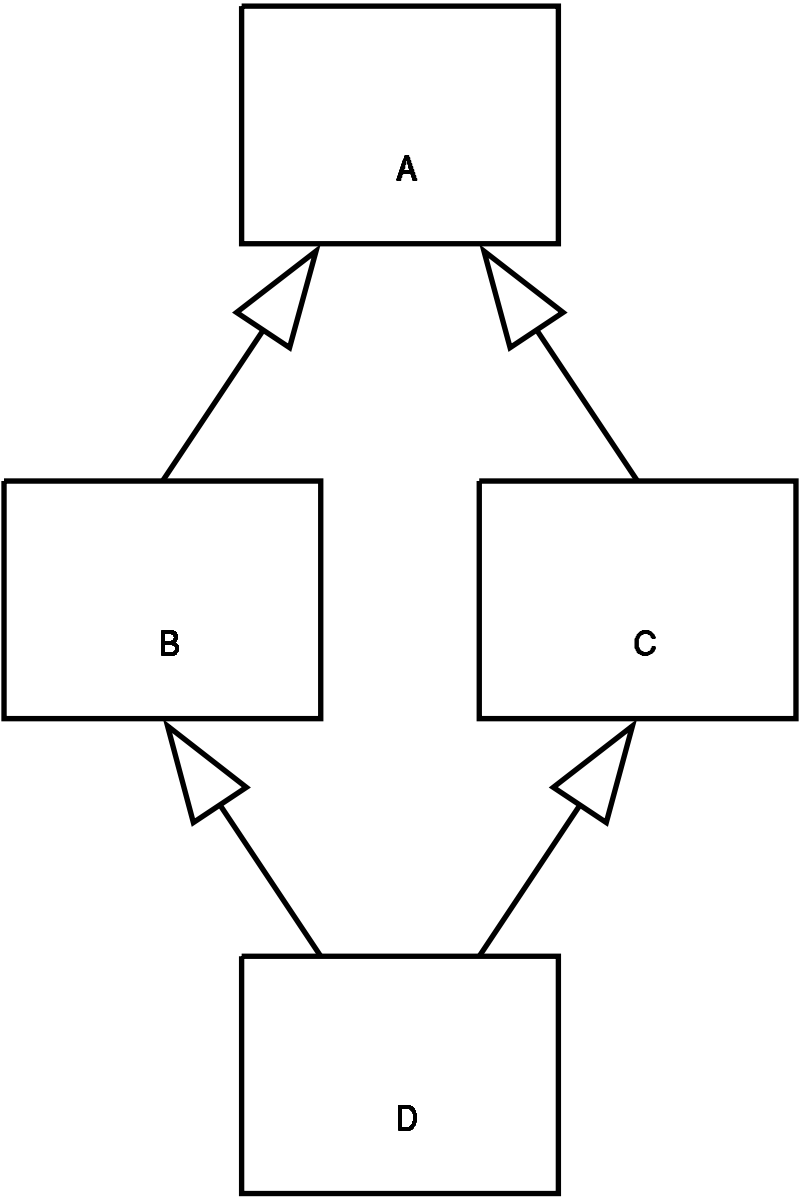
\includegraphics[width=4cm]{./immagini/diamond-inheritance.png}
\end{figure}
Siano \texttt{A}, \texttt{B}, \texttt{C}, \texttt{D} quattro classi definite nel seguente modo:
\begin{itemize}
	\item \texttt{A} possiede un metodo \texttt{doSomething()};
	\item \texttt{B}, \texttt{C} sono classi figlie di \texttt{A} che ridefiniscono entrambe tale metodo;
	\item \texttt{D} eredita sia da \texttt{B} che da \texttt{C}.
\end{itemize}
L'ambiguità si presenta dal momento in cui non è noto quale implementazione di \texttt{doSomething()} \texttt{D} erediti.
\newline
C\# e Java non adottano l'ereditarietà multipla delle classi, bensì delle \textbf{interfacce}, poiché queste ultime non specificano il comportamento di un metodo, ma solo la sua firma.
\newline
Un esempio di ereditarietà multipla delle interfacce è il seguente:
\begin{minted}
[
frame=lines,
framesep=2mm,
baselinestretch=1.2,
bgcolor=LightGray,
fontsize=\footnotesize,
linenos
]
{java}
interface flyable() {
   void fly();
}

interface swimmable() {
   void swim();
}

class Seaplane implements flyable, swimmable {
   public void fly {
	   System.out.println("I'm flying");
   }
   public void swim {
	   System.out.println("I'm swimming");
   }
}

\end{minted}
Un metodo alternativo all'ereditarietà multipla è il modello \textbf{composizione e delega}, dove si sceglie una superclasse significativa e si eredita soltanto da quella; le rimanenti superclassi diventano ruoli e vengono connesse tramite \textbf{composizione}.
Un esempio è il seguente:
\begin{itemize}
	\item Si supponga di avere la classe \texttt{Pippistrello} che eredita sia dalla classe \texttt{Mammifero} che dalla classe \texttt{Volatile}.
	\item \texttt{Mammifero} e \texttt{Volatile} ereditano da \texttt{Animale}.
	\item Dato che l'ereditarietà multipla non è consentita si può adottare il seguente approccio:
	\begin{itemize}
		\item \texttt{Animale} rimane superclasse, e \texttt{Mammifero} eredita da \texttt{Animale}.
		\item \texttt{Pippistrello} deriva da \texttt{Mammifero} ed è legato tramite composizione a \texttt{Volatile}.
	\end{itemize}
\end{itemize}
Esiste un ulteriore approccio ed è una combinazione dei metodi \textit{composizione-delega} e \textit{interfacce}.
\end{solution}


\begin{problem}{1.2}
Si esegua una classificazione del polimorfismo secondo Cardelli-Wegner e si mostri l'implementazione del polimorfismo per inclusione.
\end{problem}
\begin{solution}
Si definisce polimorfismo la capacità di un elemento di apparire in forme diverse in differenti contesti, o di elementi diversi di apparire sotto la stessa forma in uno specifico contesto.
La classificazione di Cardelli-Wegner impone due categorie, a loro volta suddivise in due sottocategorie:
\begin{itemize}
	\item \textbf{Universale}: gli elementi assumono infinite forme.
	\newline
	È suddiviso in:
	\begin{itemize}
		\item \textbf{Per inclusione}: viene utilizzato nella prorgrammazione orientata agli oggetti e utilizza:
		\begin{itemize}
			\item \textit{Overriding}: consente la ridefinizione di un metodo della superclasse nella sottoclasse. Questo approccio risulta più sicuro nel caso in cui il metodo in questione risulta astratto.
			\item \textit{Binding dinamico}: viene consentito grazie all'utilizzo della Virtual Method Table (VMT), posseduta da ogni classe; in particolare una VMT contiene tutti i puntatori ai metodi della classe che la possiede.
		\end{itemize}
		\item \textbf{Parametrico}: viene utilizzato nella programmazione generica rispetto ai tipi.
		Consiste nel definire una classe in cui il tipo di una o più variabili è un parametro della classe stessa.
		Da ogni classe generica si generano classi indipendenti, che non possiedono alcun rapporto di ereditarietà.
	\end{itemize}

	\item \textbf{Ad hoc}: gli elementi assumono un numero finito di forme.
	È suddiviso in:
	\begin{itemize}
		\item \textbf{Overloading}: consente la ridefinizione di metodi/operatori per ogni insieme di argomenti
		accettati; essa deve avvenire in fase di programmazione.

		\item \textbf{Coercion}: viene effettuata una conversione implicita del tipo di una variabile. Le conversioni possibili devono essere definite in fase
		di programmazione.

	\end{itemize}
\end{itemize}
Un esempio di polimorfismo per inclusione in cui si utilizza \textit{overriding} è il seguente:
\begin{minted}
[
frame=lines,
framesep=2mm,
baselinestretch=1.2,
bgcolor=LightGray,
fontsize=\footnotesize,
linenos
]
{csharp}
public class A {
   public virtual void Fun1(int x) {
	   ...
   }
   public virtual void Fun2(int y) {
	   ...
   }
}

public class B : A {
   public override void Fun1(int x) {
	   ...
   }
   public virtual void Fun3(int z) {
	   ...
   }
}
\end{minted}
Il codice sopra consente di mostrare un esempio di polimorfismo per inclusione: viene utilizzato \textit{overriding} per ridefinire il metodo \texttt{Fun1(int x)} della superclasse \texttt{A} in \texttt{B}.
Il \textit{binding dinamico} viene utilizzato per discriminare il metodo richiamato; la \textit{Virtual Method Table} di ciascuna classe punta al metodo evocato.
\end{solution}



\begin{problem}{1.3}
Procedimento di compilazione ed esecuzione del codice all'interno del framework .NET tramite il CLR.
\end{problem}
\begin{solution}
Il \textit{Common Language Runtime} (CLR) viene utilizzato in .NET come ambiente virtuale di esecuzione delle applicazioni.
Il codice che viene eseguito in CLR prende il nome di \textit{codice gestito}.
\newline
Il codice sorgente viene trasformato dal compilatore .NET in codice IL (CLI assembly, ovvero .exe o .dll); un assembly contiene, oltre al codice IL, anche un \textit{manifest} che fornisce informazioni come i tipi di assembly, la versione, e requisiti di sicurezza.
Il codice IL a sua volta viene convertito dal compilatore \textit{Just In Time} (JIT) in codice nativo, che può essere eseguito.
\newline
Il CLR prevede servizi aggiuntivi come:
\begin{itemize}
	\item \textbf{Garbage collector}: si occupa del ciclo di vita degli oggetti; qualora un oggetto non risulti più essere referenziato viene distrutto.
	\newline
	A differenza di \textit{Component Object Model} (COM), non viene considerato il \textit{reference counting}, ovvero il conteggio dei riferimenti a ciascun oggetto; in questo modo si ha una velocità di allocazione maggiore.
	\newline
	Sono inoltre consentiti i \textit{riferimenti circolari}, ovvero più oggetti che puntano nel seguente modo:
	\begin{figure}[h]
	\centering
	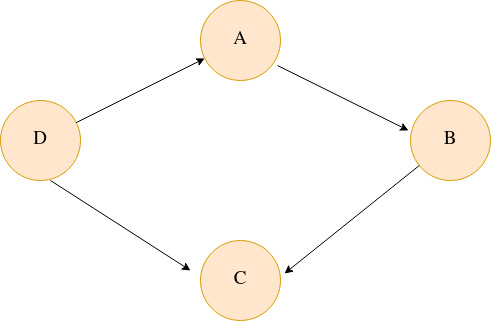
\includegraphics[width=6cm]{./immagini/riferimentiCircolari.jpg}
	\caption{Riferimenti circolari}
\end{figure}\\
	Con questo approccio, tuttavia, si verifica la perdita della \textit{distruzione deterministica}, ovvero una richiesta esplicita di liberazione della memoria occupata da un oggetto.
	\\Tramite \textit{garbage collector} la memoria viene liberata in modo non deterministico, ovvero quando l'oggetto non risulta più raggiungibile.
	\item \textbf{I/O su file};
	\item \textbf{Gestione delle eccezioni}: le eccezioni sono oggetti che ereditano dalla classe \textit{System.Exception}.
	\newline
	È possibile gestire le eccezioni sfruttando i seguenti tre concetti:
	\begin{itemize}
		\item \textit{throw}: lancio di un'eccezione;
		\item \textit{catch}: cattura di un'eccezione;
		\item \textit{finally}: esecuzione di codice di uscita da un blocco controllato.
	\end{itemize}
\end{itemize}
\end{solution}

\begin{problem}{1.4}
Differenza tra tipi valore e tipi riferimento in .NET
\end{problem}
\begin{solution}
I \textit{Common Type System} (CTS) sono tipi di dato supportati dal framework .NET, che forniscono un modello di programmazione unificato ai linguaggi orientati agli oggetti, funzionali e procedurali.
In CTS tutte le classi ereditano da \texttt{System.Object}, ed esistono due categorie di tipi:
\begin{itemize}
	\item \textbf{Tipi riferimento}: sono indirizzi di memoria che rappresentano i riferimenti agli oggetti allocati sull'heap gestito.
	\item \textbf{Tipi valore}: sono allocati sullo stack, o appartengono ad altri oggetti, e contengono direttamente un valore (ovvero una sequenza di byte).
	\newline
	I tipi valore includono:
	\begin{itemize}
		\item \textbf{Tipi primitivi}: Int32, double, decimal, char, boolean, etc.
		\item \textbf{Tipi definiti dall'utente}: strutture dati ed enumerativi.
	\end{itemize}
\end{itemize}
È possibile eseguire conversioni da tipo valore a tipo riferimento mediante un \textit{up cast} \textbf{implicito} a \\\texttt{System.Object}: questa procedura prende il nome di \textit{boxing}:
\begin{center}
\texttt{double d = 333.3;}
\\
\texttt{Object obj = d;}
\end{center}
L'\textit{unboxing}, operazione inversa al \textit{boxing}, permette di convertire un tipo riferimento a un tipo valore, tramite un \textit{down cast} \textbf{esplicito}:
\begin{center}
	\texttt{double d2 = (double)obj;}
\end{center}
Il passaggio dei parametri a un metodo può avere risultati distinti, in base alla tipologia di oggetto passato come argomento.
Esistono tre tipologie di argomenti:
\begin{itemize}
	\item \textbf{In}
	\begin{itemize}
		\item \textit{Tipi valore}: si ha passaggio per copia dell'oggetto e la modifica da parte del metodo invocato avviene solo sulla copia.
		\item \textit{Tipi riferimento}: si ha passaggio per copia del riferimento dell'oggetto, e la modifica da parte del metodo invocato avviene sulla copia del riferimento, ma non sul riferimento originale.
	\end{itemize}
	In entrambi i casi gli argomenti passati ai metodi devono essere stati già inizializzati.
	Un esempio è il seguente:
	\begin{minted}
[frame=lines,
framesep=2mm,
baselinestretch=1.2,
bgcolor=LightGray,
fontsize=\footnotesize,
linenos
]
{csharp}

PostoRistorante posto = new PostoRistorante(1,1);
assegnaPosto(ref posto);
Console.writeline(posto); // sia se PostoRistorante è una classe si ha (3,5)
			// se è una struttura si ha (1,1)

static void assegnaPosto(ref PostoRistorante posto){
	posto.NumeroTavolo = 3;
	posto.NumeroPosto = 5;
}
	\end{minted}
	\item \textbf{In/Out}
	\begin{itemize}
		\item \textit{Tipi valore}: si ha passaggio per riferimento e le modifiche influenzano l'oggetto originale.
		\item \textit{Tipi riferimento}: si ha passaggio per riferimento dell'\textit{indirizzo dell'oggetto} e le modifiche influenzano l'oggetto referenziato, ma non l'oggetto originale.
	\end{itemize}
	In entrambi i casi gli argomenti passati ai metodi devono essere stati già inizializzati.
	\begin{minted}
[frame=lines,
framesep=2mm,
baselinestretch=1.2,
bgcolor=LightGray,
fontsize=\footnotesize,
linenos
]
{csharp}

PostoRistorante posto = new PostoRistorante(1,1);
assegnaPosto(ref posto);
Console.writeline(posto); // sia se PostoRistorante è una classe,
			// sia se è una struttura si ha (3,5)

static void assegnaPosto(ref PostoRistorante posto){
	posto.NumeroTavolo = 3;
	posto.NumeroPosto = 5;
}
	\end{minted}
	\item \textbf{Out}: si ha passaggio, sia per gli oggetti di tipo riferimento che di tipo valore, dei loro indirizzi, e le modifiche hanno effetto sul chiamante.
	\newline
	L'inizializzazione degli oggetti deve avvenire nel metodo in cui sono stati passati come argomenti.
	Un esempio è il seguente:
	\begin{minted}
[frame=lines,
framesep=2mm,
baselinestretch=1.2,
bgcolor=LightGray,
fontsize=\footnotesize,
linenos
]
{csharp}

PostoRistorante posto;
assegnaPosto(out posto);

static void assegnaPosto(out PostoRistorante posto){
	posto = new PostoRistorante(3,5);
}
	\end{minted}
\end{itemize}
\end{solution}


\begin{problem}{1.5}
Garbage Collector in C\#
\end{problem}
\begin{solution}
Il \textit{Garbage Collector} si occupa del rilascio delle risorse qualora esse non vengano più utilizzate da un oggetto.
Consente di avere maggiore stabilità del programma, poiché evita che un programmatore manipoli direttamente puntatori ad aree di memoria.
\newline
Il vantaggio dell'utilizzo di un garbage collector è il contrasto delle seguenti problematiche:
\begin{itemize}
	\item \textbf{Dangling pointer}: puntatori ad aree di memoria deallocate precedentemente, che potrebbero essere state successivamente assegnate a un altro oggetto.
	\item \textbf{Doppia deallocazione}: causata da più chiamate consecutive di deallocazione della stessa area di memoria.
	\item \textbf{Memory leak}: un oggetto non più utilizzato non viene deallocato, pertanto continua a occupare memoria.
\end{itemize}
Gli svantaggi invece sono:
\begin{itemize}
	\item vengono richieste maggiori risorse di calcolo;
	\item incertezza del momento in cui viene effettuata la garbage collection;
	\item il rilascio della memoria è non deterministico, ovvero non si sa il momento esatto in cui il rilascio avviene, né l'ordine di rilascio delle aree non più utilizzate. Ciò può dipendere dall'algoritmo utilizzato dal garbage collector.
\end{itemize}
L'ambiente .NET sfrutta come strategia di \textit{garbage collection} il \textbf{tracing}: si stabiliscono quali oggetti sono raggiungibili e si eliminano quelli non raggiungibili.\newline
Quando un processo viene inizializzato il \textit{Common Language Runtime} (CLR) riserva una regione contigua di spazio di indirizzamento, noto come \textit{managed heap} e memorizza l'indirizzo di partenza della regione in un puntatore chiamato \texttt{NextObjPtr}.
Nel caso in cui venga eseguita una \textit{newobj}, il CLR:
\begin{enumerate}
	\item Determina la dimensione in byte dell'oggetto e aggiunge a quest'ultimo due campi che possono essere da 32 o 64 bit.
	Il primo campo contiene un puntatore alla tabella dei metodi, mentre il secondo è un campo \texttt{SyncBlockIndex}.
	\item Controlla se a partire da \texttt{NextObjPtr} ci sia spazio sufficiente; in caso negativo viene utilizzato il Garbage Collector, o viene lanciata \texttt{OutOfMemoryException}.
	\item Aggiorna i puntatori relativi all'oggetto appena creato e allo spazio libero di memoria:
	\begin{center}
		\texttt{thisObjPtr = NextObjPtr;}

		\texttt{NextObjPtr += sizeof(oggetto);}

	\end{center}
	\item Invoca il costruttore dell'oggetto.
	\item Restituisce il riferimento all'oggetto.
\end{enumerate}
Lo scopo del garbage collector è di individuare quali oggetti non vegono più utilizzati dall'applicazione; quest'ultima presenta un insieme di radici (\textit{root}).
Ciascuna radice è un puntatore a un oggetto di tipo riferimento sicuramente attivo, come:
\begin{itemize}
	\item variabili globali e field statici di tipo riferimento;
	\item variabili locali o argomenti attuali di tipo riferimento presenti sugli stack dei vari thread;
	\item registri della CPU contenenti gli indirizzi di oggetti di tipo riferimento.
\end{itemize}
Vengono distinte di tipologie di oggetti: gli \textbf{oggetti vivi} sono raggiungibili (direttamente o indirettamente) dalle radici, mentre gli \textbf{oggetti garbage} non lo sono.
\newline
Inizialmente il garbage collector marca tutti gli oggetti sul \textit{managed heap} come \textbf{garbage}; successivamente viene interpellata la tabella delle radici, per stabilire quali oggetti siano \textbf{vivi}, marcandoli come tali.
\newline
Terminata la classificazione degli oggetti viene liberata la memoria occupata dagli oggetti garbage; tuttavia ciò causa frammentazione nel managed heap, poichè si hanno aree di memoria libere non contigue.
Pertanto si effettua una compattazione della memoria in uso, modificando di conseguenza i riferimenti agli oggetti spostati; al termine dell'unificazione si aggiorna il valore di \texttt{NextObjPtr}.
\\\\
Il Garbage collector può effettuare tutte le operazioni elencate in precedenza, in quanto conosce il tipo di un oggetto e può sfruttare i metadati per determinare quali campi dell'oggetto contengono riferimenti agli altri oggetti.
\newline
Nel caso in cui un oggetto contenga riferimenti a risorse di tipo unmanaged (file, connessione al database, socket, e così via) è responsabilità del programmatore occuparsi della fase di finalizzazione, ovvero il rilascio della risorsa prima della deallocazione.
\end{solution}


\begin{problem}{1.6}
Passaggio dei parametri in C\#
\end{problem}
\begin{solution}
	Il passaggio dei parametri a un metodo può avere risultati distinti, in base alla tipologia di oggetto passato come argomento.
Esistono tre tipologie di argomenti:
\begin{itemize}
	\item \textbf{In}
	\begin{itemize}
		\item \textit{Tipi valore}: si ha passaggio per copia dell'oggetto e la modifica da parte del metodo invocato avviene solo sulla copia.
		\item \textit{Tipi riferimento}: si ha passaggio per copia del riferimento dell'oggetto, e la modifica da parte del metodo invocato avviene sulla copia del riferimento, ma non sul riferimento originale.
	\end{itemize}
	In entrambi i casi gli argomenti passati ai metodi devono essere stati già inizializzati.
	Un esempio è il seguente:
	\begin{minted}
[frame=lines,
framesep=2mm,
baselinestretch=1.2,
bgcolor=LightGray,
fontsize=\footnotesize,
linenos
]
{csharp}

PostoRistorante posto = new PostoRistorante(1,1);
assegnaPosto(ref posto);
Console.writeline(posto); // sia se PostoRistorante è una classe si ha (3,5)
			// se è una struttura si ha (1,1)

static void assegnaPosto(ref PostoRistorante posto){
	posto.NumeroTavolo = 3;
	posto.NumeroPosto = 5;
}
	\end{minted}
	\item \textbf{In/Out}
	\begin{itemize}
		\item \textit{Tipi valore}: si ha passaggio per riferimento e le modifiche influenzano l'oggetto originale
		\item \textit{Tipi riferimento}: si ha passaggio per riferimento dell'\textit{indirizzo dell'oggetto} e le modifiche influenzano l'oggetto referenziato, ma non l'oggetto originale
	\end{itemize}
	In entrambi i casi gli argomenti passati ai metodi devono essere stati già inizializzati.
	\begin{minted}
[frame=lines,
framesep=2mm,
baselinestretch=1.2,
bgcolor=LightGray,
fontsize=\footnotesize,
linenos
]
{csharp}

PostoRistorante posto = new PostoRistorante(1,1);
assegnaPosto(ref posto);
Console.writeline(posto); // sia se PostoRistorante è una classe,
			// sia se è una struttura si ha (3,5)

static void assegnaPosto(ref PostoRistorante posto){
	posto.NumeroTavolo = 3;
	posto.NumeroPosto = 5;
}
	\end{minted}
	\item \textbf{Out}: si ha passaggio, sia per gli oggetti di tipo riferimento che di tipo valore, dei loro indirizzi, e le modifiche hanno effetto sul chiamante.
	\newline
	L'inizializzazione degli oggetti deve avvenire nel metodo in cui sono stati passati come argomenti.
	Un esempio è il seguente:
	\begin{minted}
[frame=lines,
framesep=2mm,
baselinestretch=1.2,
bgcolor=LightGray,
fontsize=\footnotesize,
linenos
]
{csharp}

PostoRistorante posto;
assegnaPosto(out posto);

static void assegnaPosto(out PostoRistorante posto){
	posto = new PostoRistorante(3,5);
}
	\end{minted}
\end{itemize}
\end{solution}




\begin{problem}{1.7}
Concetto di delegato in C\#
\end{problem}
\begin{solution}
I delegati sono oggetti che contengono un riferimento a un metodo da invocare.
\newline
Sono equivalenti ai puntatori a funzioni (\textit{functor}) presenti nei linguaggi C/C++, ma orientati agli oggetti ed efficaci.
\newline
Eseguono funzionalità di \textit{callback}, tra le quali:
\begin{itemize}
	\item \textbf{Elaborazione asincrona}: permette a un metodo di accettare un delegato come parametro e di chiamare il delegato in un momento successivo. Questo tipo di elaborazione viene eseguita quando un processo impiega molto tempo ad essere completato; quando viene terminato il chiamante viene avvertito.
	\item \textbf{Elaborazione cooperativa}: viene fornita una parte del servizio dal metodo \textbf{chiamato} e la parte rimanente viene effettuata dal \textbf{chiamante}.
	\newline
	Un esempio di elaborazione cooperativa è il \textit{merge sort}.
	\item \textbf{Gestione degli eventi}: ogni entità interessata a un determinato evento si registra presso il generatore dell'evento, specificando quale metodo gestirà l'evento.
\end{itemize}
L'istanza di un delegato può incapsulare uno o più metodi, specificando gli argomenti di ciascun metodo e il valore restituito.
Ciascun metodo è riferito a un'entità richiamabile che può essere:
\begin{itemize}
	\item un metodo, nel caso di metodi statici;
	\item un'istanza e il metodo relativo a quell'istanza, nel caso di istanze di metodi.
\end{itemize}
Un delegato contiene soltanto la firma del metodo, e non conosce la classe o il metodo a cui si sta riferendo; è quindi ideale per l'invocazione anonima.
Nel caso in cui si abbia l'invocazione di un'istanza delegata, che possiede una o più voci nell'elenco di invocazione, si invocano i metodi dell'elenco in ordine e in modo sincrono.
Il delegato è inoltre un’entità type-safe che si pone tra un chiamante e zero o più \textit{call target} e che si comporta come
un’interfaccia con un solo metodo.
Per ciascun metodo invocato vengono passati come argomenti gli stessi forniti all'istanza del delegato. Si hanno due scenari:
\begin{itemize}
	\item Nel caso in cui vengono inclusi \textbf{parametri di riferimento} nell'invocazione del delegato, ciascuna invocazione del metodo avviene con un riferimento alla medesima variabile e le modifiche alla variabile da parte di un metodo nell'elenco di invocazione saranno visibili ai metodi successivi nell'elenco di invocazione.
	\item Nel caso di invocazione del delegato con \textbf{parametri di output} o \textbf{valori di ritorno} il loro valore finale sarà determinato dall'invocazione dell'ultimo delegato presente nell'elenco.
\end{itemize}
Un esempio di utilizzo di delegati è il seguente:
\begin{itemize}
	\item Si ha un impiegato che deve effettuare una specifica attività
	\item Si ha un capo, il cui scopo è di controllare l'attività dei suoi impiegati
	\item Un impiegato deve comunicare al suo capo l'inizio dell'attività, lo svolgimento e l'eventuale conclusione: per farlo sfrutta un delegato che contiene un riferimento alle sue attività.
\end{itemize}
\end{solution}

\begin{problem}{1.8}
Concetto di evento in C\#
\end{problem}
\begin{solution}
Un evento viene utilizzato al posto di un delegato in quanto quest’ultimo utilizza campi pubblici per la registrazione di
metodi.
\newline
\texttt{Event} consente di rendere automatico il supporto per la pubblica registrazione e l’implementazione privata.
\newline
Si possono fornire gestori di registrazione eventi definiti dall’utente: un possibile vantaggio di questo approccio è il
\textit{controllo}.
\newline
Un evento viene scaturito dall’interazione con l’utente o in seguito alla logica del programma.
Esistono tre entità relative agli eventi:
\begin{itemize}
	\item \textbf{Event sender}: la sorgente dell’evento è l’oggetto o la classe che scaturisce l’evento.
	\item \textbf{Event receiver}: l’oggetto o la classe per il quale l’evento è determinante e quindi desidera di venire notificato
   in caso di verifica dell’evento
	\item \textbf{Event handler}: il metodo dell’\textit{event receiver}, eseguito nel momento in cui avviene la notifica.
\end{itemize}
Quando un evento si verifica, il sender invia un messaggio di notifica a tutti i \textit{receiver}; in genere il \textit{sender} non ha modo
di conoscere né i gli \textit{handler}, né i \textit{receiver} e grazie all’utilizzo di delegati si collegano \textit{sender} e \textit{receiver}, consentendo
\textit{invocazioni anonime}.
L’evento incapsula il delegato, pertanto occorre dichiarare un tipo di delegato prima di dichiarare un evento.
I delegati possiedono due parametri:
\begin{itemize}
	\item la fonte che ha scatenato l’evento;
	\item dati dedicati all’evento.
\end{itemize}
Molti eventi non possiedono dati, pertanto è sufficiente utilizzare il delegato presente nella classe
\\\texttt{System.EventHandler}. Occorre definire nuovi delegati per gestire gli eventi soltanto quando questi ultimi possiedono
dei dati.
Nel caso in cui un evento non debba passare ulteriori informazioni ai propri gestori viene sfruttata la classe
\texttt{System.EventArgs}, aggiungendo i dati necessari e utilizzando il delegato \texttt{EventHandler<TEventArgs>}.
\\
Nel caso in cui si dichiari un evento, come
\begin{center}
	\texttt{Public event EventHandler changed}
\end{center}
La keyword \texttt{event} ne limita sia le possibilità di utilizzo che la visibilità; successivamente l’evento viene trattato come
un delegato di tipo speciale, e può diventare \texttt{null} se nessun cliente si è registrato; può venire associato a uno o più
metodi da invocare.
\\
Dato che un evento può essere visto come un delegato, sono consentite soltanto alcune operazioni del delegato,
come l’aggiunta di un delegato all’evento (grazie all’operatore \texttt{+=}) oppure sganciarsi da un evento (mediante
l’operatore \texttt{-=}).
\\
Per ricevere notifiche relative a quell’evento occorre che il cliente definisca un metodo \texttt{EventHandler}, che verrà
evocato all’atto della notifica dell’evento; dopodiché si crea un delegato dello stesso tipo dell’evento, viene riferito al
metodo e successivamente lo si aggiunge alla lista dei delegati di quell’evento.
\\Grazie alle singole operazioni \texttt{+=} e \texttt{-=} ammesse nessuno può ottenere o modificare l’elenco dei metodi sottostante dei
gestori di eventi.

\end{solution}
\begin{problem}{1.9}
Metaprogrammazione e riflessione in C\#
\end{problem}
\begin{solution}
La metaprogrammazione viene utilizzata per programmare  un sistema in modo che abbia accesso alle informazioni relative al sistema stesso, e che possa manipolare tali informazioni.
Essa viene realizzata mediante la \textbf{riflessione}, implementata in C\# tramite la classe \texttt{System.Reflection}.
La riflessione sfrutta i \textbf{metadati}, ovvero dati che descrivono altri dati; infatti, se un componente dispone di informazioni sufficienti per descrivere se stesso, le sue interfacce possono essere esplorate dinamicamente.
In Java e .NET i dati sono generati nel momento in cui si definisce un tipo, vengono salvati assieme alla sua definizione e sono disponibili a \textit{runtime}; in COM e CORBA i metadati sono definiti da \textit{Interface Definition Language} (IDL).
La riflessione viene utilizzata per:
\begin{itemize}
	\item esaminare i dettagli di un \textit{assembly};
	\item istanziare oggetti e chiamare metodi scoperti a runtime;
	\item creare, compilare ed eseguire assembly, ove necessario.
\end{itemize}
La chiave per la \textit{riflessione} in .NET è la classe \texttt{System.Type}:
\begin{itemize}
	\item tutti gli oggetti sono istanze di tipi, e i tipi stessi sono istanze di \texttt{System.Type};
	\item il tipo di un oggetto può essere scoperto tramite il metodo \texttt{GetType()};
	\item è presente un solo oggetto \texttt{Type} per ogni tipo definito.
\end{itemize}
Ad esempio, è possibile enumerare i tipi di un \textit{assembly} tramite i seguenti comandi:
\begin{itemize}
	\item \texttt{Assembly.Load(...)} restituisce un oggetto \texttt{Assembly};
	\item \texttt{Assembly.GetModules(...)} restituisce un array di oggetti \texttt{Module};
	\item \texttt{Module.GetTypes(...)} restitusice un array di \texttt{Type}.
\end{itemize}
È possibile creare istanze di tipi e accedere ai loro membri mediante \textit{very late binding}:
\begin{itemize}
	\item \texttt{Activator.CreateInstance(type, ...)} invoca il costruttore specificato;
	\item \texttt{methodInfo.Invoke(...)} invoca i metodi;
	\item \texttt{propertyInfo.GetValue(...)/.SetValue(...)} invocano \textit{getter} e \textit{setter}.
\end{itemize}
I membri pubblici sono sempre accessibili, mentre i membri non pubblici lo sono solo se il chiamante ha permessi sufficienti.
Per creare dinamicamente istanze di oggetti si usa la classe \texttt{System.Activator}, il cui metodo \texttt{CreateInstance(Type type, Object[] args)} è equivalente all'operazione \texttt{new}.
\newline\newline
Per aggiungere informazioni ai metadati è possibile utilizzare \textbf{attributi personalizzati}, ovvero classi visibili via riflessione che derivano da \texttt{System.Attribute} e che possono contenere proprietà e metodi.
\newline
Per creare attributi personalizzati occorre:
\begin{itemize}
	\item dichiarare la classe dell'attributo;
	\item dichiarare i costruttori;
	\item dichiarare le proprietà;
	\item opzionalmente applicare \texttt{AttributeUsageAttribute}, che specifica alcune caratteristiche della classe, ovvero a quali elementi l'attributo è applicabile, quando l'attributo può essere ereditato e quando possono esistere molteplici istanze di un attributo.
\end{itemize}
Il metodo \texttt{GetCustomAttributes()} restituisce la lista degli attributi personalizzati.
\newline
La classe \texttt{System.Reflection.Emit} consente di scrivere il codice IL necessario per creare e compilare un \textit{assembly} che potrà essere chiamato direttamente dal programma che lo ha creato, e che potrà essere archiviato su disco in modo che altri programmi possano utiizzarlo.
\end{solution}


\begin{problem}{1.10}
Spiegare i quattro bad design (fragilità, immobilità, rigidità, viscosità)
\end{problem}
\begin{solution}
La qualità del design risulta fondamentale per rendere un programma:
\begin{itemize}
	\item maggiormente affidabile;
	\item maggiormente efficiente;
	\item maggiormente manutenibile;
	\item maggiormente economico.
\end{itemize}
Esistono quattro principi che peggiorano la qualità del software:
\begin{enumerate}
	\item \textbf{Rigidità del software}: rende complesse le modifiche al software, in quanto una piccola modifica influenza gran parte del programma, a causa di modifiche a cascata su moduli dipendenti tra loro.
	\newline Una conseguenza di questo principio è la grande quantità di tempo necessaria a gestire una modifica del software.
	\item \textbf{Fragilità del software}: responsabile del malfunzionamento del software di fronte a una modifica di quest'ultimo; il software risulta difficile da mantenere, in quanto per ogni correzione è presente un rischio maggiore di guasto.
	\item \textbf{Immobilità del software}: rende il software inutilizzabile da parti dello stesso progetto o da altri progetti; ciò avviene quando un modulo software è fortemente dipendente da altri moduli.
	\newline Di conseguenza occorre scrivere nuovo software, anziché riutilizzarlo.
	\item \textbf{Viscosità del software}: questo principio favorisce l'utilizzo di \textit{hack}, ovvero soluzioni funzionanti, ma che snaturano il design, in quanto non seguono le \textit{best practice}.
	\newline
	La viscosità è maggiormente presente nel caso in cui utilizzo di hack risulta molto più semplice di una soluzione che preserva la progettazione iniziale.
	\newline
	Esistono due categorie di viscosità:
	\begin{itemize}
		\item \textbf{Viscosità del design}: l'utilizzo di metodi che rispettino il design risulta più complesso che utilizzare hack.
		\item \textbf{Viscosità dell'ambiente}: l'ambiente di sviluppo è lento e inefficiente: si possono avere tempi di compilazione molto lunghi, il sistema di controllo del codice sorgente richiede ore per la registrazione di pochi file.
	\end{itemize}
\end{enumerate}
I motivi di una progettazione non corretta sono dovuti a:
\begin{itemize}
	\item incapacità dei progettisti nel seguire le \textit{best practice};
	\item limiti imposti dall'esterno, in termini di tempo e risorse;
	\item pratiche obsolete;
	\item evoluzione del progetto: in seguito a cambiamenti dei requisiti e modifiche al software, non si ha più la manutenibilità del progetto originario.
\end{itemize}
\end{solution}


\begin{problem}{1.11}
Principio di singola responsabilità con almeno un esempio
\end{problem}
\begin{solution}
Il principio di singola responsabilità afferma che ogni elemento di un programma (classe, metodo, variabile) deve avere un'unica responsabilità, interamente gestita dall'elemento stesso.
Tutti i servizi offerti dall'elemento stesso dovrebbero essere allineati a tale responsabilità.
\newline
Una responsabilità risulta un motivo per cambiare, e ogni classe o modulo deve avere un solo motivo per cambiare.
\newline
Il principio prevede di sviluppare classi o moduli indipendenti tra loro e semplici.
Un esempio di applicazione del seguente principio è il seguente:
\begin{itemize}
	\item si ha una classe \texttt{MacchinaFotografica}:
	\item \texttt{MacchinaFotografica} possiede due funzionalità indipendenti tra loro, ovvero \texttt{Foto} e \texttt{Video};
	\item unire le due funzionalità in un'unica classe risulta poco portabile e la modifica a una funzionalità influenza l'altra, pertanto si creano due classi separate \texttt{Fotocamera} e \texttt{Videocamera}.
\end{itemize}
\end{solution}


\begin{problem}{1.12}
Principio di inversione delle dipendenze con almeno un esempio
\end{problem}
\begin{solution}
Il principio di inversione delle dipendenze prevede che i moduli di alto livello (i \textit{clienti}) non debbano dipendere dai moduli di basso livello (i \textit{fornitori dei servizi}). Entrambi devono dipendere da \textit{astrazioni}.
\newline
Il motivo della precedente affermazione è dovuto alla presenza di codice e della logica implementativa nei moduli di basso livello. Nel caso in cui i moduli di alto livello dovessero dipendere da moduli di basso livello si avrebbe:
\begin{itemize}
	\item \textbf{Rigidità}: per ogni modifica occorre intervenire su un numero elevato di moduli.
	\item \textbf{Fragilità}: per ogni modifica verrebbero introdotti errori nel sistema.
	\item \textbf{Immobilità}: non è possibile riutilizzare il codice, in quanto i moduli di alto livello non si riuscirebbero a separarare da quelli di basso livello.
\end{itemize}
Con il principio di inversione delle dipendenze si eviterebbero i problemi sopra elencati, in quanto le astrazioni possiedono poco codice e sono poco soggetti a modifiche; inoltre è presente una separazione tra moduli astratti e moduli concreti, che permette modifiche limitate al modulo concreto interessato (poiché nessuno dipende da questi moduli).
Dato che i dettagli del sistema sono stati isolati da un muro di astrazioni stabili:
\begin{itemize}
	\item i cambiamenti non possono più propagarsi (\textit{design for change});
	\item i singoli moduli sono maggiormente riusabili (\textit{design for resue}).
\end{itemize}
Un esempio di principio di inversione delle dipendenze è il seguente:
\begin{itemize}
	\item Si considerino le classi concrete \texttt{BigliettoNormale} e \texttt{GestoreVenditaBiglietti}; quest'ultima ha una dipendenza verso \texttt{BigliettoNormale}.
	\item Tale dipendenza è verso una classe concreta, pertanto il codice di \texttt{GestoreVenditaBiglietti} è poco manutenibile.
	\newline Infatti, nel caso si volesse creare la classe \texttt{BigliettoVIP} occorrerebbe modificare il codice di \\\texttt{GestoreVenditaBiglietti}.
	\item Per risolvere il problema, si introduce l'interfaccia \texttt{IBiglietto} e si fa sì che \texttt{GestoreVenditaBiglietti} dipenda da essa; inoltre, si modifica la classe \texttt{BigliettoNormale} in modo che implementi \texttt{IBiglietto}.
	\item A questo punto, se si volesse aggiungere una nuova tipologia di biglietto, non sarebbe più necessario modificare \texttt{GestoreVenditaBiglietti} ma basterebbe creare una classe concreta che implementi \texttt{IBiglietto} (ad esempio, \texttt{BigliettoVIP}).
\end{itemize}
\end{solution}


\begin{problem}{1.13}
Principio di segregazione delle interfacce con almeno un esempio
\end{problem}
\begin{solution}
Questo principio prevede che un cliente non debba dipendere dai metodi che non usa, e che quindi è preferibile avere più interfacce specifiche, anzichè una sola interfaccia con più funzioni (\textit{fat interface}).
\newline
Nel caso di utilizzo delle \textit{fat interfaces} sarà più difficile mantenere il sistema, in quanto è rappresentato da un unico blocco; pertanto occorre creare interfacce specifiche per ogni cliente.
\newline
Un esempio di mancato utilizzo di principio di segregazione delle interfacce è la creazione, da parte di Xerox (creatore dello standard \textit{Ethernet}), di una stampante avente diverse funzionalità, tra cui mandare fax e pinzare fogli. Le modifiche al software, sebbene piccole, risultavano difficili, in quanto tutte le diverse funzioni eseguite dalla stampante multi-uso erano implementate all'interno di una sola classe.
Tramite l'utilizzo del principio di segregazione delle interfacce si avevano più interfacce, ciascuna specifica per il ruolo della stampante, come ad esempio le interfacce \texttt{IScanFogli} e \texttt{IPinzaFogli}.
\\
Ciacsuna modifica di una funzione risulta più semplice, in quanto \textit{autocontenuta}.
\end{solution}


\begin{problem}{1.14}
Principio aperto/chiuso con almeno un esempio
\end{problem}
\begin{solution}
Il principio aperto/chiuso prevede un sistema aperto a estensioni software, ma chiuso a modifiche.
\newline
Per realizzare questo principio vengono utilizzate classi astratte e interfacce; nel caso in cui si vogliano aggiungere nuove funzionalità sarà necessario, anzichè modificare il codice, creare una nuova classe concreta che implementi le astrazioni.
\newline
Per soddisfare il principio aperto/chiuso si occorre all’ereditarietà:
\begin{itemize}
	\item \textbf{di interfaccia}: le classi derivate ereditano da una classe base astratta con
	funzioni virtuali. In questo modo l’interfaccia è chiusa alle modifiche e il suo comportamento può
	essere modificato implementando nuove classi derivate.
	\item \textbf{dell’implementazione}: si creano nuove sottoclassi che estendono la classe base, mantenendo il codice comune in quest'ultima.
	\newline
	In questo modo si evitano ripetizioni nelle sottoclassi.
\end{itemize}


Questo approccio consente una maggiore modularità del sistema e stabilità, in quanto non si modificano componenti definite precedentemente e non si introducono eventuali errori dovuti alle modifiche.
Un esempio di utilizzo OCP è il seguente:
\begin{itemize}
	\item Si supponga di avere una classe \texttt{CalcolatoreSpeseAziendali} la quale, data una collezione di oggetti di tipo \texttt{Impiegato}, restituisca le spese totali dovute al loro salario, tramite metodo\\ \texttt{CalcolaSpese(Collection<Impiegato> impiegati)}.
	\item Si definisce un'interfaccia o una classe astratta \texttt{Impiegato} che espone il metodo \texttt{getSalario()}.
	\item Si definiscono le classi concrete \texttt{Manager}, \texttt{AmministratoreDelegato}, \texttt{Programmatore} che implementano \texttt{Impiegato} e che possiedono un salario specifico al ruolo ricoperto.
	\item A questo punto \texttt{CalcolaSpese(Collection<Impiegato> impiegati)} attraverserà la collezione e sommerà i salari dei vari dipendenti, senza conoscere il loro ruolo.
	\item Di conseguenza, in caso venga aggiunto un nuovo ruolo come \texttt{Venditore} con OCP non sarà necessario modificare il codice, ma soltanto aggiungere una nuova classe e ridefinire il metodo \texttt{getSalario()} al suo interno.
\end{itemize}
\end{solution}


\begin{problem}{1.15}
Principio di sostituibilità di Liskov con almeno un esempio
\end{problem}
\begin{solution}
Il principio di sostituibilità di Liskov definisce il rapporto tra una classe e le relative sottoclassi.
Esistono due versioni di questo principio:
\begin{itemize}
	\item \textbf{Versione debole}: a ogni riferimento della classe base (classe padre) deve essere associata l'istanza della sottoclasse (classe figlia).
	\item \textbf{Versione forte}: ogni programma che utilizza istanze della classe base non percepisce variazioni logiche nell'utilizzo delle istanze delle relative sottoclassi.
\end{itemize}
Per essere più specifici, occorre introdurre due concetti definiti dal \textit{design by contract}:
\begin{itemize}
	\item \textbf{Precondizioni}: requisiti minimi che devono essere soddisfatti dal chiamante, affinchè il metodo invocato possa essere eseguito correttamente.
	\item \textbf{Postcondizioni}: requisiti soddisfatti dal metodo chiamato, nel caso di esecuzione corretta.
\end{itemize}
Per ogni metodo re-implementato dalla sottoclasse:
\begin{itemize}
	\item le precondizioni devono essere ugualmente o meno stringenti;
	\item le postcondizioni devono essere ugualmente o più stringenti;
	\item la semantica della classe base deve essere conservata;
	\item non è possibile aggiungere vincoli alla classe base.
\end{itemize}
Ad esempio, data la classe \texttt{Uccello} dotata del metodo \texttt{vola()} si hanno i due seguenti scenari:
\begin{itemize}
	\item la sottoclasse \texttt{Pinguino}, che eredita da \texttt{Uccello}, presenta una violazione del principio di sostituibilità di Liskov, in quanto l'utilizzo del metodo \texttt{vola()} deve essere ridefinito, senza mantenere la semantica (ad esempio sollevando un'eccezione, dato che un pinguino non può volare).
	\item la sottoclasse \texttt{Piccione}, che eredita da \texttt{Uccello}, non presenta una violazione del principio di sostituibilità di Liskov, in quanto la semantica del metodo \texttt{vola()} viene rispettata.
\end{itemize}
\end{solution}


\begin{problem}{1.16}
Principi per l'architettura dei package
\end{problem}
\begin{solution}
L'architettura dei package prevede i seguenti tre principi:
\begin{itemize}
	\item \textbf{Principio di equivalenza di riuso/rilascio (REP)}: un elemento riutilizzabile deve essere periodicamente fornito e rilasciato da un sistema apposito, poiché chi rilascia il software non è la stessa persona che lo utilizza.
	\newline
	Se non è garantita la manutenzione del software l'utilizzo di quest'ultimo non dovrebbe essere permesso ai clienti. Occorre pertanto raggruppare le classi in \textit{package}, in modo da modo da garantire il riutilizzo di una o più classi.
	\item \textbf{Principio di chiusura comune (CCP)}: occorre ridurre al minimo l'utilizzo di \textit{package}, in modo che risulti più semplice gestire e modificare ciascuna classe e ridustribuire ciascun package.
	\newline
	Occorre quindi raggruppare più classi che vengono modificate insieme nello stesso \textit{package}.
	\item \textbf{Principio di riutilizzo comune (CRP)}: occorre non raggruppare nello stesso package le classi che non vengono riutilizzate insieme.
	\newline La motivazione è dovuta al fatto che, per ciascuna modifica del package, sia necessario controllare ogni singola classe per verificare il corretto funzionamento dell'aggiornamento; vengono controllate anche le classi che non presentano alcuna modifica.
\end{itemize}
Risulta complesso soddisfare tutti e tre i principi contemporaneamente, poichè il \textit{principio di chiusura comune} suggerisce di rendere i package \textbf{i più grandi possibili}, semplificando l'utilizzo di questi ultimi da parte dello sviluppatore, mentre il \textit{principio di equivalenza di riuso/rilascio} e il \textit{principio di riutilizzo comune} incentivano l'utilizzo di \textbf{package piccoli}, semplificandone l'utilizzo da parte dei clienti.
\\
Una buona prassi è applicare il \textit{principio di chiusura comune} durante la progettazione dell'architettura, in modo da semplificare lo sviluppo e la manutenzione. Una volta ottenuta maggiore stabilità del sistema viene eseguito un \textit{refactoring}, diminuendo i package e soddisfando i rimanenti due principi per permettere maggiore riutilizzo.
\newline
\newline
Sono presenti ulteriori tre principi che descrivono le relazioni tra i \textit{package}:
\begin{itemize}
	\item \textbf{Principio delle dipendenze acicliche (ADP)}: afferma che non devono essere presenti dipendenze tra package che possano creare dei cicli.
	Nel caso in cui si voglia modificare una classe occorre ricompilare l'intero package di appartenenza e i package che dipendono da quest'ultimo; nel caso di dipendenza ciclica una modifica di una classe potrebbe portare a ricompilare l'intero progetto.
	\newline
	Per evitare questo problema occorre introdurre un'interfaccia per la classe responsabile delle dipendenze cicliche, e sfruttando il \textit{principio di inversione delle dipendenze}, oppure trasferire le dipendenze in un nuovo package.
	\item \textbf{Principio delle dipendenze stabili (SDP)}: stabilisce che un package dovrebbe dipendere soltanto da package più stabili di esso.
	\newline
	Un package stabile rispetta il principio di chiusura comune, poiché le modifiche a una classe non causano effetti a cascata sull'intero progetto, bensì rimangono interne al package di appartenenza.
	\item \textbf{Principio delle astrazioni stabili:} i package stabili dovrebbero essere astratti, poiché facili da estendere. Un package astratto non contiene codice soggetto a modifiche.
\end{itemize}
Occorre inoltre considerare i sistemi di package a livelli: i package nei livelli superiori sono instabili e facilmente modificabili, mentre nei livelli inferiori sono presenti package difficilmente modificabili.
Una buona prassi consiste nel possedere package stabili \textbf{astratti}, in modo che risultino difficili da modificare, ma facili da estendere (sfruttando il principio aperto/chiuso).

\end{solution}

\newpage
\begin{problem}{1.17}
Pattern Singleton con esempi
\end{problem}
\begin{solution}
Il pattern Singleton prevede che una classe abbia una sola istanza; chiunque può accedervi attraverso l'unica istanza citata.
Una classe che implementa il pattern Singleton è strutturata nel sequente modo:
\begin{minted}
[
frame=lines,
framesep=2mm,
baselinestretch=1.2,
bgcolor=LightGray,
fontsize=\footnotesize,
linenos
]
{java}
public class Singleton {

   private static Singleton istance = null; // riferimento all' istanza

   private Singleton() {} // costruttore

   public static Singleton getIstance() {
	if (istance == null)
	   istance = new Singleton();
    return istance;
   }

   public void metodo() { ... }

}

\end{minted}
Il costruttore è privato, in quanto assicura che viene creata al più un'istanza della classe \texttt{Singleton}.
Il metodo statico \texttt{getInstance()} controlla se è già esistente un'istanza della classe: in caso affermativo restituisce l'istanza creata in precedenza, altrimenti crea una nuova istanza.
\newline
Una classe con soli membri statici non rappresenta un'alternativa al pattern Singleton, in quanto non permette di creare istanze personalizzate in base al contesto; non permette inoltre di utilizzare un numero arbitrario di interfacce.
\newline
Un esempio di utilizzo del pattern Singleton è l'accesso a un database, in quanto si vuole garantire atomicità.
\begin{figure}[h]
    \centering
    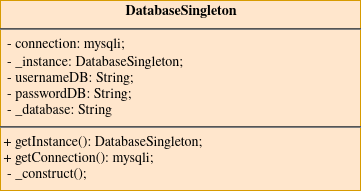
\includegraphics[scale=0.5]{./immagini/DatabaseSingleton.png}
  \end{figure}
\end{solution}

\begin{problem}{1.18}
Pattern Observer con esempi
\end{problem}
\begin{solution}
Il pattern \textit{Observer} viene utilizzato nel caso in cui un oggetto (detto \textit{subject}) debba notificare un cambiamento del proprio stato interno a uno o più oggetti (detti \textit{observer}).
Si definiscono le seguenti classi:
\begin{itemize}
	\item \texttt{Subject} dichiara i metodi \texttt{Attach()} (o \texttt{Register()}), \texttt{Detach()} (o
	\texttt{Unregister()}) e \texttt{Notify()}.
	\item Gli Observer dichiarano il metodo \texttt{Update()}.
\end{itemize}
Per registrarsi presso \textit{Subject}, un \textit{Observer} invoca il metodo \texttt{Attach()}.
Successivamente, in caso di evento, \textit{Subject} chiama il metodo \texttt{Notify()}, che esegue \texttt{Update()} di tutti gli Observer che si sono registrati.
\\Infine, un \texttt{Observer} si può disiscrivere a un \texttt{Subject}, sfruttando il metodo \texttt{Detach()}.
\newline
Il pattern Observer è una delle cinque possibili soluzioni nel caso in cui si voglia aggiornare elementi in base al cambiamento del \textit{subject}.
Altri possibili quattro approcci sono:
\begin{itemize}
	\item \textbf{Class based}: Ogni subject ha un riferimento diretto all'observer da notificare
	\item \textbf{Interface based}: Ogni subject possiede un riferimento all'interfaccia implementata dagli \textit{observer}, aumentando il disaccoppiamento tra subject e observer
	\item \textbf{Delegate based}: Ogni subject contiene un delegato pubblico, in modo che gli observer possano registrarsi a tale delegato e venire notificati indirettamente dal subject
	\item \textbf{Event based}: un event si occupa di effettuare \texttt{Unregister()} degli observer.
\end{itemize}
Un esempio di utilizzo di pattern Observer potrebbe essere l'iscrizione da parte di diversi dispositivi elettronici a un sensore di temperatura; nel caso in cui la temperatura della stanza cambi, tutti i dispositivi registrati al subject \texttt{Sensore} vengono avvertiti.
\newline
\newline
\textbf{Diagramma UML:}
\begin{figure}[htb!]
	\centering
	\label{ObserverPattern}
	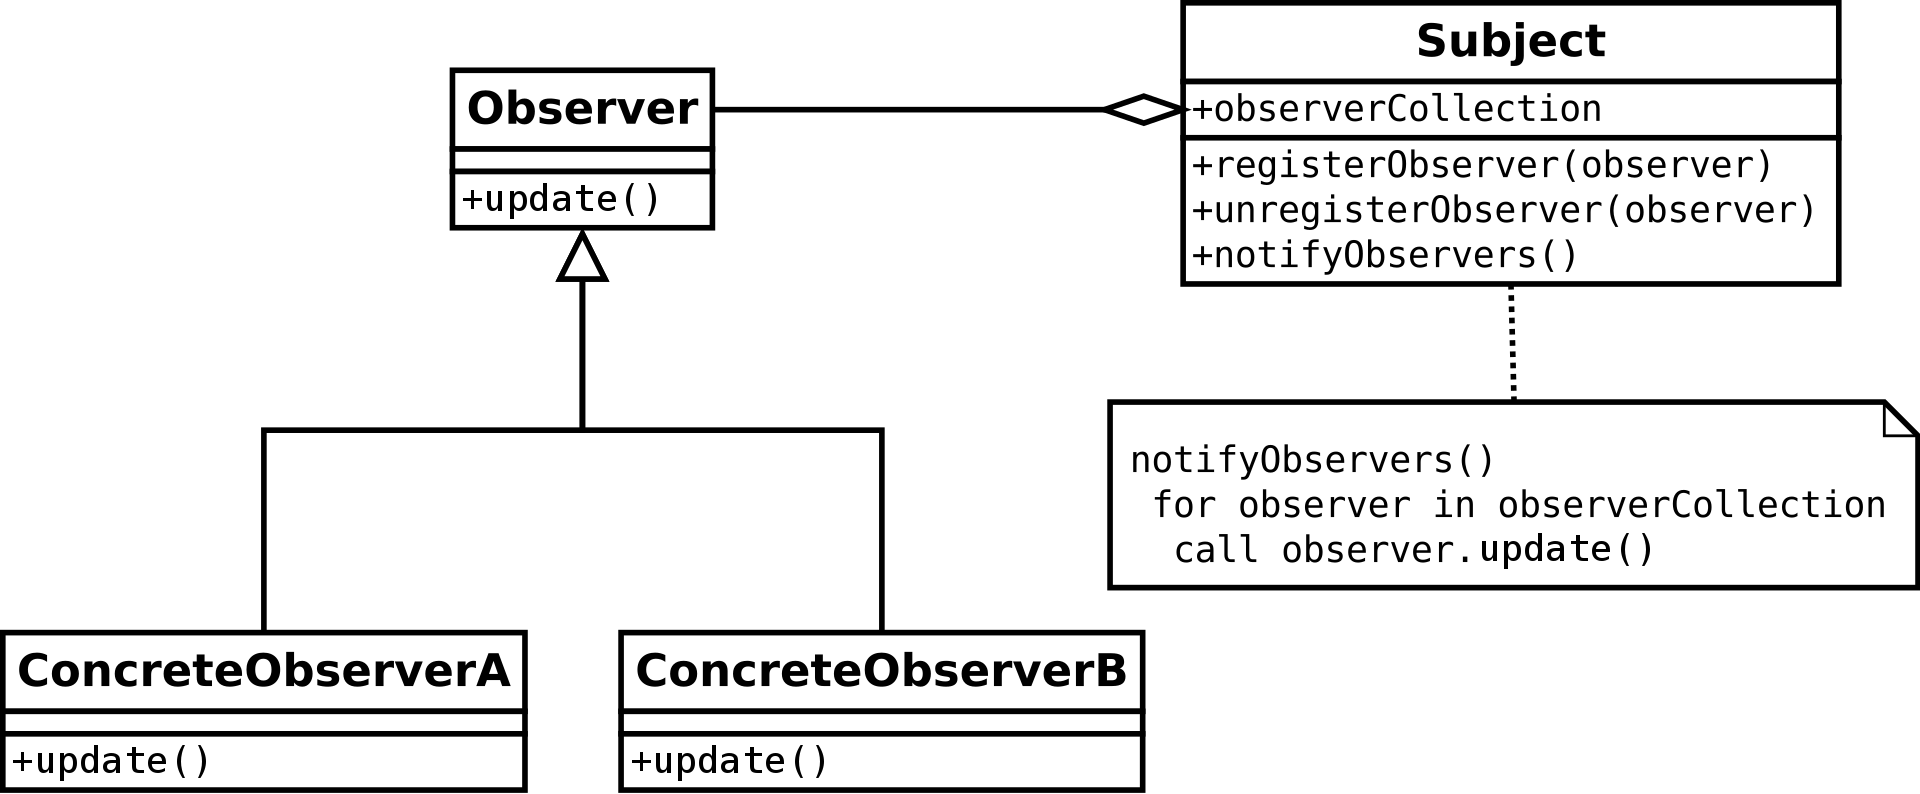
\includegraphics[width=9cm]{./immagini/observerPattern.png}
\end{figure}
\end{solution}

\begin{problem}{1.18.1}
Pattern Flyweight con esempi
\end{problem}
\begin{solution}
Il pattern \textit{Flyweight} consente la condivisione di oggetti leggeri tra più entità, in modo tale che il loro utilizzo non sia troppo costoso.
L'oggetto condiviso (\texttt{flyweight}) viene utilizzato da più client in modo efficace nello stesso momento.
In particolare:
\begin{itemize}
	\item l'oggetto non deve essere distinguibile da un oggetto non condiviso;
	\item l'oggetto non deve fare ipotesi sul contesto in cui opera.
\end{itemize}
Una corretta condivisione dei \textit{flyweight} tra i clienti viene garantita dall'utilizzo di \textit{FlyweightFactory}.
Esistono due stati associati al pattern:
\begin{itemize}
	\item \textbf{intrinseco}: stato memorizzato in \texttt{flyweight} e non dipende dal contesto di utilizzo
	\item \textbf{estrinseco}: stato memorizzato dal cliente, dipende dal contesto di utilizzo e non può essere condiviso da tutti i clienti.
	Viene passato a \texttt{flyweight} da parte del client quando viene invocata una operazione relativa a flyweight.
\end{itemize}
Un esempio di pattern \textit{Flyweight} potrebbe essere la rappresentazione dei caratteri in un \textit{word processor}:
\begin{itemize}
	\item Si consideri la classe \texttt{Carattere}. Senza pattern \textit{flyweight} ogni carattere scritto dall'utente risulterebbe in un nuovo oggetto \texttt{Carattere}, causando un'alta occupazione di memoria.
	\item Applicando il pattern \textit{flyweight} si riutilizza lo stesso carattere, senza ridefinire un nuovo oggetto a ogni sua occorrenza.
	\item La classe \texttt{Carattere} può contenere i campi nome, font, dimensione, che rappresentano lo stato intrinseco dell'oggetto \texttt{Flyweight}.
	\item Lo stato estrinseco è rappresentato dalla posizione del carattere (come riga e colonna) all'interno del testo, pertanto va gestito dal \textit{client}.
\end{itemize}
\newpage
\textbf{Diagramma UML:}
\begin{figure}[htb!]
	\centering
	\label{FlyweightPattern}
	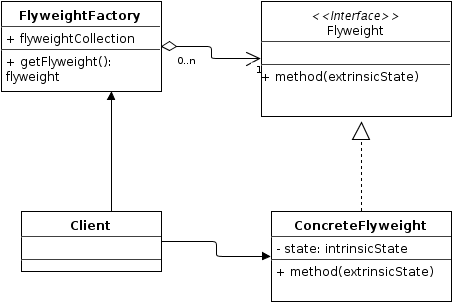
\includegraphics[width=8cm]{./immagini/flyweightPattern.png}
\end{figure}
\end{solution}

\begin{problem}{1.19}
Pattern Strategy con esempi
\end{problem}
\begin{solution}
Il pattern \textit{Strategy} è un pattern di tipo comportamentale e viene utilizzato quando si ha una famiglia di algoritmi, intercambiabili tra loro, che implementano una determinata funzionalità.
A questo scopo si dichiara un'interfaccia dotata di metodi che svolgono la funzionalità richiesta; si dichiara inoltre, per ogni algoritmo, una classe concreta che implementa l'interfaccia e i relativi metodi definiti precedentemente.
\newline
Nel caso in cui un \textit{cliente}, che dipende unicamente dall'interfaccia, voglia eseguire le relative funzionalità, non deve fare assunzioni su quale strategia sia stata adottata.
\newline
Un esempio di utilizzo del pattern Strategy è il seguente:
\begin{itemize}
	\item Interfaccia \texttt{ISortStrategy} che espone il metodo \texttt{sort()}.
	\item Classe concreta \texttt{MergeSortStrategy} che implementa l'interfaccia \texttt{ISortStrategy} e realizza il metodo \texttt{sort()}, usando l'algorirmo di \textit{merge sort}.
	\item Classe concreta \texttt{QuickSortStrategy} che implementa l'interfaccia \texttt{ISortStrategy} e realizza il metodo \texttt{sort()}, usando l'algorirmo di \textit{quick sort}.
	\item Classe concreta \texttt{BubbleSortStrategy} che implementa l'interfaccia \texttt{ISortStrategy} e realizza il metodo \texttt{sort()}, usando l'algorirmo di \textit{bubble sort}.
	\item Classe \texttt{Cliente} che ha un riferimento a un oggetto di tipo \texttt{ISortStrategy}.
\end{itemize}
\textbf{Diagramma UML:}
\begin{figure}[htb!]
	\centering
	\label{StrategyPattern}
	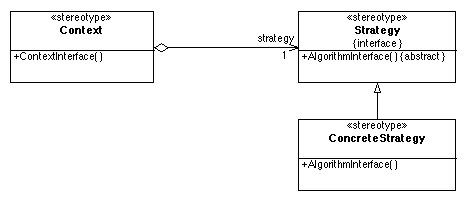
\includegraphics[width=10cm]{./immagini/strategyPattern.png}
\end{figure}
\end{solution}


\begin{problem}{1.20}
Pattern Adapter con esempi
\end{problem}
\begin{solution}
Il pattern \textit{Adapter} è un pattern di tipo strutturale.
Si supponga che un Cliente dipenda da un'interfaccia Target già definita, la quale espone un certo metodo.
Esiste una certa classe \texttt{Adaptee} che realizza tale metodo, ma ha un'interfaccia incompatibile con l'interfaccia \texttt{Target}.
Di conseguenza, per risolvere questo problema, si utilizza una classe Adapter, che implementa Target e richiama il metodo di \texttt{Adaptee}, mascherandolo come una chiamata al metodo di \texttt{Target}.
Un esempio di utilizzo del pattern Adapter è il seguente:
\begin{itemize}
	\item Si ha un'interfaccia MediaPlayer che espone il metodo play().
	\item Si ha una classe MP3Player fornita da una libreria esterna, che riproduce file di tipo MP3, e che non è compatibile con MediaPlayer.
	\item Si ha una classe Cliente che richiede un servizio a MediaPlayer per riprodurre un file di tipo MP3.
	\item Si realizza una classe MediaAdapter, che implementa MediaPlayer e che mantiene un riferimento a MP3Player; in particolare quando il client einvocherà il metodo play() di MediaPlayer, verrà invocato da MediaAdapter il metodo play() di MP3Player, senza che il cliente se ne accorga.
\end{itemize}
\textbf{Diagramma UML:}
\begin{figure}[htb!]
	\centering
	\label{ObserverPattern}
	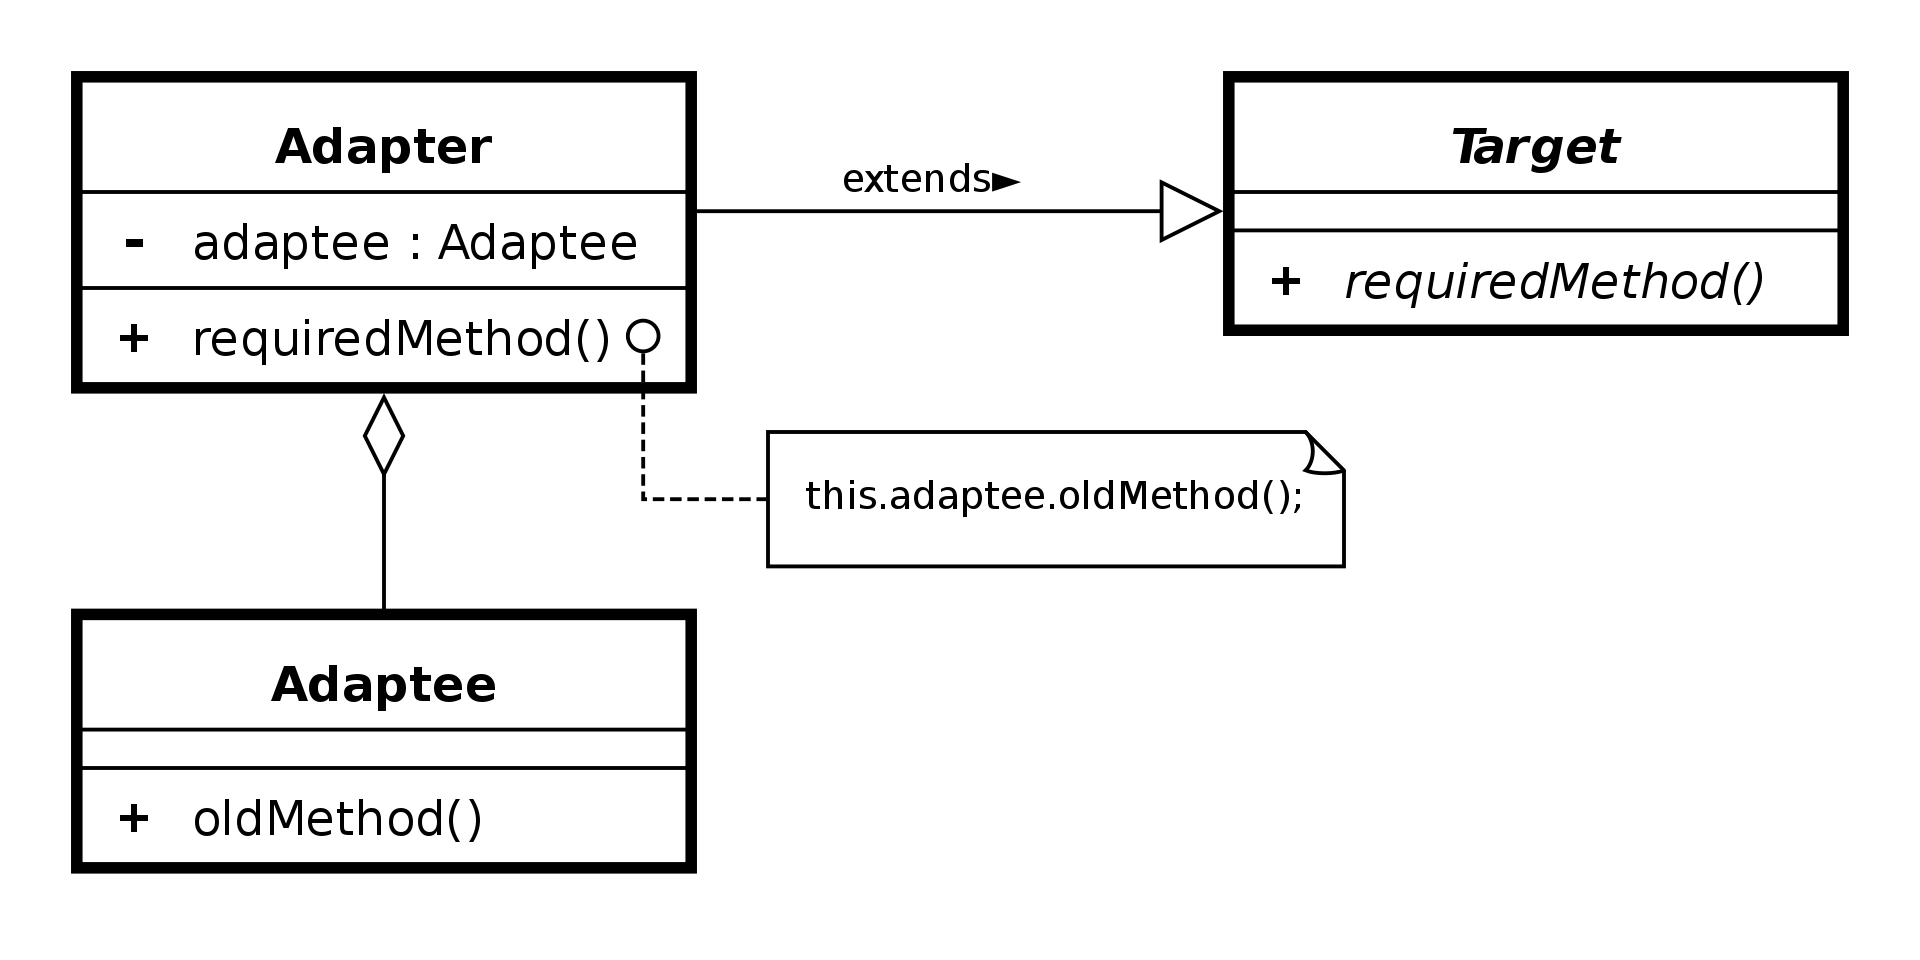
\includegraphics[width=9cm]{./immagini/adapterPattern.png}
\end{figure}
\end{solution}


\begin{problem}{1.21}
Pattern Decorator con esempi
\end{problem}
\begin{solution}
Il pattern \textit{Decorator} è un pattern di tipo strutturale.
Consente di aggiungere dinamicamente responsabilità a un oggetto, e risulta essere una valida alternativa all'ereditarietà, qualora si abbia una gerarchia troppo estesa.
I vantaggi del pattern \textit{Decorator} rispetto all'ereditarietà sono i seguenti:
\begin{itemize}
	\item Consente di aggiungere dinamicamente nuove funzionalità a un oggetto a \textit{run-time}, mentre l'ereditarietà estende il comportamento delle classi padre alle classi figlie durante la fase di compilazione
	\item Codice pulito e più semplice da testare
\end{itemize}
In particolare viene soddisfatto il principio di singola responsabilità, in quanto il pattern \textit{Decorator} permette di suddividere una funzionalità in più classi che svolgono uno specifico compito.
\newline
Si supponga di avere una classe \texttt{Component} che rappresenta l'interfaccia dell'oggetto a cui aggiungere dinamicamente nuove funzionalità, e la classe \texttt{ConcreteComponent} che rappresenta l'oggetto in questione.
Per aggiungere la funzionalità all'oggetto si dichiara una classe astratta \texttt{Decorator}, che mantiene un riferimento all'oggetto \texttt{Component} e definisce un' interfaccia ad esso conforme, e una classe \texttt{ConcreteDecorator} che rappresenta l'oggetto che aggiunge nuove funzionalità a \texttt{ConcreteComponent}
Un esempio di utilizzo del pattern \textit{Decorator} è il seguente:
\begin{itemize}
\item Si ha un'interfaccia \texttt{ITea} che rappresenta \texttt{Component}
\item Si hanno le classi \texttt{GreenTea}, \texttt{BlackTea} che implementano l'interfaccia \texttt{ITea}, e rappresentano i
\\
\texttt{ConcreteComponent}
\item Si vuole dare la possibilità di aggiungere ulteriori ingredienti in ciascun tè; pertanto si dichiara la classe astratta \texttt{TeaExtra}, che rappresenta il \texttt{Decorator};
\item Si realizzano le classi che concretizzano la classe \texttt{TeaExtra}, come \texttt{TeaWithMilk}, \texttt{TeaWithHoney},
\\
\texttt{TeaWithIce}
\end{itemize}
\textbf{Diagramma UML:}
\begin{figure}[htb!]
	\centering
	\label{ObserverPattern}
	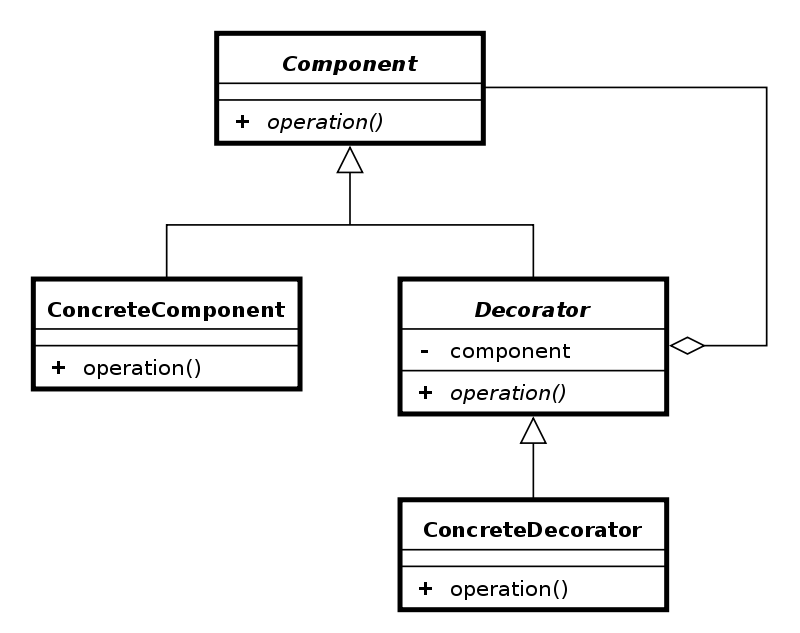
\includegraphics[width=9cm]{./immagini/decoratorPattern.png}
\end{figure}
\end{solution}

\begin{problem}{1.22}
Pattern Composite con esempi
\end{problem}
\begin{solution}
Il pattern \textit{composite} è un pattern di tipo strutturale.\newline
Nasce per facilitare la manipolazione delle strutture ad albero, che risulta essere complessa e prona ad errori, poiché bisogna distinguere tra un nodo (oggetto composto) e una foglia (oggetto singolo).
La soluzione al problema citato è la definizione di un'interfaccia che permetta di trattare allo stesso modo oggetti singoli e composti.
Per realizzare il pattern \textit{composite} si suppone di avere le seguenti componenti:
\begin{itemize}
	\item \texttt{Component}: classe astratta che dichiara un'interfaccia che consente l'accesso e la manipolazione degli oggetti della composizione.
	\item \texttt{Client}: accede agli oggetti che derivano da \texttt{Component} e li manipola attraverso l'interfaccia di
	\\\texttt{Component}.
	\item \texttt{Leaf}: descrive il comportamento degli oggetti singoli, ovvero le foglie, e che non possono avere figli.
	\item \texttt{Composite}: definisce il comportamento degli oggetti aventi figli.
\end{itemize}
È necessario che il contenitore dei figli sia un attributo di \texttt{Composite}, e può essere di qualsiasi tipo (come array, lista,
hashtable ecc).
Il \texttt{Client} utilizza soltanto \texttt{Component}, pertanto quest'ultimo deve possedere tutti i metodi di cui il \texttt{Client} necessita e la definizione base dei metodi che dovranno essere ridefiniti dalle sottoclassi.
Alcune operazioni definite in \texttt{Component} risultano prive di significato per gli oggetti senza figli, come \texttt{add}, \texttt{remove}, pertanto sono possibili due possibili approcci:

\begin{itemize}
\item \textbf{Trasparenza}: si definiscono le operazioni di \texttt{add} e \texttt{remove} in \texttt{Component}.
Tuttavia è possibile che il \texttt{Client} definisca operazioni illegali come l'aggiunta di figli alle foglie; per evitare questo problema è necessario che le foglie sollevino eventualmente un'eccezione per i metodi precedentemente citati.
	\item \textbf{Sicurezza}: i metodi di gestione dei figli come \texttt{add} e \texttt{remove} vengono implementati in \texttt{Composite}; occorre predisporre di un'implementazione che verifichi se l'oggetto che si sta trattando è un \texttt{Composite} o \texttt{Leaf}.
\end{itemize}
Un esempio di utilizzo del pattern \textit{composite} è il seguente:
\begin{itemize}
\item Si supponga di avere come \texttt{Client} un oggetto che deve accedere alla gerarchia di impiegati di un'azienda informatica.
\item Si ha una classe astratta \texttt{Impiegato}, che rappresenta il \texttt{Component}.
\item Si consideri la classe \texttt{Manager}, che rappresenta \texttt{Composite}, e che può avere come sottoposti altri impiegati.
\item Si consideri la classe \texttt{Programmatore}, che rappresenta \texttt{Leaf} e che non ha sottoposti.
\item Una eventuale operazione di \texttt{aggiungiSottoposto()} può essere eseguita da \texttt{Manager}, ma non da
\\
\texttt{Programmatore}.
\end{itemize}
\textbf{Diagramma UML:}
\begin{figure}[htb!]
	\centering
	\label{ObserverPattern}
	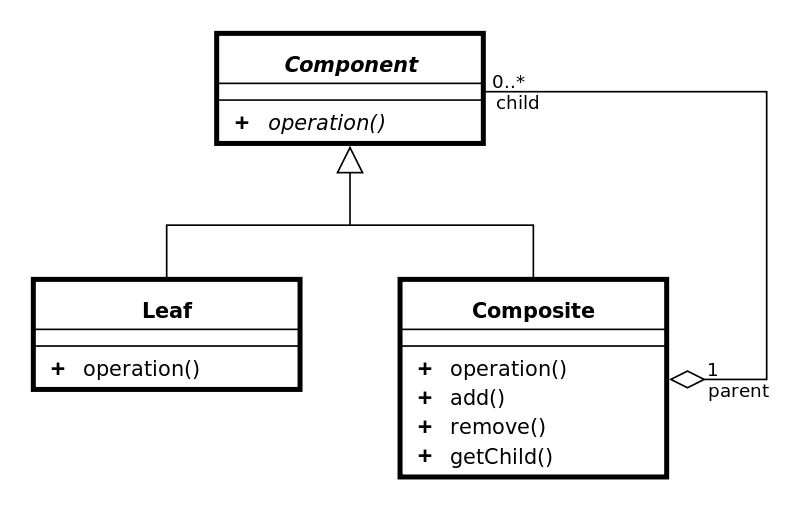
\includegraphics[width=9cm]{./immagini/compositePattern.png}
\end{figure}
\end{solution}


\begin{problem}{1.23}
Pattern Visitor con esempi
\end{problem}
\begin{solution}
Il pattern \textit{Visitor} è un pattern comportamentale che separa in un'apposita classe l'operazione relativa a una struttura di oggetti.
\newline
In questo modo è possibile l'aggiunta di nuove operazioni definendo appositamente delle classi; non vengono quindi modificate le classi appartententi a una struttura che utilizzerà le nuove operazioni.
Vengono soddisfatti due principi:
\begin{itemize}
\item il principio aperto/chiuso, in quanto l'intero sistema è aperto per aggiungere nuove funzionalità, ma risulta chiuso alle modifiche.
\item il principio di singola responsabilità, poiché ogni funzionalità è in un'apposita classe.
\end{itemize}
Per realizzare il pattern \textit{visitor} si suppone di avere le seguenti componenti:
\begin{itemize}
	\item \textbf{Visitor}: classe astratta o un'interfaccia, che dichiara il metodo \texttt{VisitElement}.
	\item \textbf{ConcreteVisitor}: classe concreta che estende o implementa \texttt{Visitor} e che consente di percorrere la struttura di oggetti coinvolta.
	\item \textbf{Element}: classe astratta o interfaccia che dichiara il metodo \texttt{Accept}, che ha come parametro un oggetto di tipo \texttt{Visitor}.
	\item \textbf{ConcreteElement}: classe concreta che estende o implementa \texttt{Element}.
	\item \textbf{ObjectStructure}: è realizzata come \textit{Composite} o come una collezione (array, lista, etc.) e deve contentire l'enumerazione dei suoi elementi ; per permettere di essere visitabile da \texttt{Visitor}, \texttt{ObjectStructure} deve implementare un'interfaccia apposita \texttt{Visitable}.
\end{itemize}
Occorre considerare i seguenti aspetti:
\begin{itemize}
	\item Per definire una nuova operazione occorre implementare un nuovo \texttt{ConcreteVisitor}; quest'ultimo, durante un'operazione, può modificare il proprio stato.
	\item Per permettere a un \texttt{Visitor} l'accesso allo stato degli elementi della struttura, è necessario sfruttare
	\\l'\textbf{incapsulamento}.
	\item La gerarchia composta da \texttt{Element} deve essere stabile, poichè non è semplice aggiungere nuovi \\\texttt{ConcreteElement}: ciò implicherebbe definire in tutti i \texttt{Visitor} esistenti un metodo apposito \texttt{visit} per quel \texttt{ConcreteElement}.
	\item L'operazione \texttt{Accept} è di tipo \textit{double dispatch}, poiché dipende sia da \texttt{Visitor} che da \texttt{Element}.
\end{itemize}
Si consideri il seguente esempio:
\begin{itemize}
	\item Si suppone di avere un negozio che vende libri e CD musicali.
	\item Si definisce la classe \texttt{Negozio} che contiene una collezione di elementi.
	\item Si definisce una classe astratta \texttt{Elemento}, che presenta il metodo \texttt{accept(Visitor v)}, e le classi concrete \texttt{Libro} e \texttt{CD}, che derivano da \texttt{Elemento}.
	\item Si definisce l'interfaccia \texttt{Visitor} che presenta i metodi \texttt{visitLibro(Libro libro)} e \texttt{visitCD(CD cd)}.
	\item Si definisce la classe \texttt{VisitorVendita}, che implementa visitor e che racchiude rispettivamente la logica di vendita di libri e CD nei metodi \texttt{visitLibro(Libro libro)} e \texttt{visitCD(CD cd)}.
	\item Il negozio vuole consentire il prestito di libri e CD; per farlo sarà sufficiente creare una classe\\\texttt{VisitorPrestito}, che implementa \texttt{Visitor} e ridefinisce i metodi \texttt{visitCD} e \texttt{visitLibro}.
\end{itemize}

\textbf{Diagramma UML:}
\begin{figure}[htb!]
	\centering
	\label{ObserverPattern}
	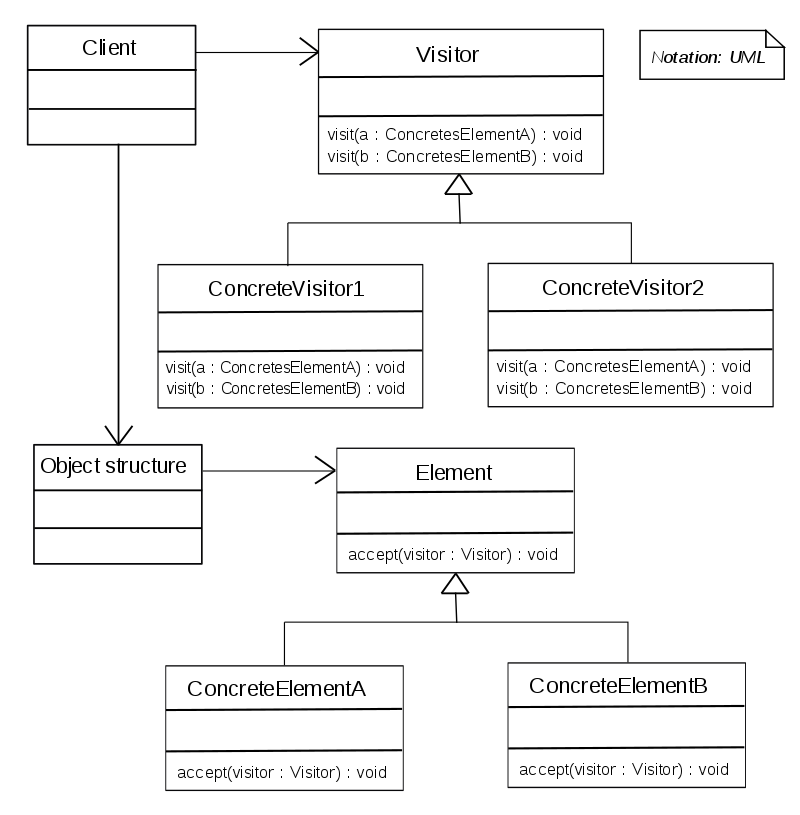
\includegraphics[width=8cm]{./immagini/visitorPattern.png}
\end{figure}
\end{solution}


\begin{problem}{1.24}
Modello LMU nei VCS con vantaggi e svantaggi
\end{problem}
\begin{solution}
Il modello \textit{Lock-Modify-Unlock} (LMU) viene utilizzato in alcuni sistemi di controllo delle versioni e consente a una sola persona alla volta di modificare file di una \textit{repository}.
Ogni volta che un utente voglia modificare un determinato file della cartella di lavoro deve prima \textbf{bloccarlo} (\textit{lock}); una volta completata la modifica occorre \textbf{sbloccare} il file.
Questo modello presenta diversi svantaggi:
\begin{itemize}
	\item Esiste la possibilità che un utente si dimentichi di sbloccare il file, non consentendo a nessun altro di modificare il file.
	\newline
	Si generano quindi notevoli ritardi nello sviluppo.
	\item Si crea una serializzazione non necessaria, poiché la modifica contemporanea dello stesso file da parte di due persone non implica la generazione di conflitti.
	\item È presente un falso senso di sicurezza da parte degli sviluppatori nel blocco di un file: nel caso in cui un utente modifichi un file, e un altro utente apporti cambiamenti su un secondo file si possono generare conflitti se i due file hanno dipendenze tra loro.
	\newline
	A causa dei conflitti generati i due file non funzionano più correttamente insieme.
	\item Il lavoro può esssere eseguito soltando offline.
\end{itemize}
Un vantaggio che il modello offre è la possibilità di lavoro nel caso in cui si hanno file non unibili, come ad esempio i file immagine
\end{solution}


\begin{problem}{1.25}
Modello CMM nei VCS con vantaggi e svantaggi
\end{problem}
\begin{solution}
Il modello \textit{Copy-Modify-Merge} viene utilizzato in alcuni sistemi di controllo delle versioni e prevede l'assenza di meccanismi di blocco dei file in caso di modifica (\textit{lock}).
Ogni client dell'utente esegue l'accesso alla \textit{repository} del progetto e crea una copia personale e locale su cui lavorare. Gli utenti possono lavorare indipendentemente e in parallelo, modificando le loro copie private.
Nel momento del \textit{check in}, le modifiche effettuate da un utente al progetto vengono unite alle modifiche degli altri utenti: l'operazione appena descritta prende il nome di \textit{merge}.
L'operazione appena descritta può avere due esiti:
\begin{itemize}
	\item \textbf{Successo}: le modifiche effettuate non causano problemi di congruenza del codice
	\item \textbf{Conflitto}: due o più utenti hanno modificato lo stesso blocco di codice, generando incongruenze.
	\newline
	In questo caso occorre risolvere i conflitti a mano.
\end{itemize}
Anche in caso di conflitto il tempo di risoluzione del problema risulta minore rispetto al ritardo di sviluppo introdotto da un sistema di blocco come previsto nel modello \textit{Lock-Modify-Unlock}.
L'assenza di conflitti non garantisce sempre il corretto funzionamento del programma dopo le modifiche: l'operazione di \textit{merge} infatti non è in grado di rilevare conflitti logici, concettuali o semantici.
\end{solution}

\newpage
\section{Modulo 2}
\begin{problem}{2.1}
Spiegare il modello a cascata e le sue criticità.
\end{problem}
\begin{solution}
Il modello a cascata (waterfall model) è un modello di processo di sviluppo software che prevede fasi sequenziali distinte tra loro:
\begin{itemize}
	\item studio di fattibilità;
	\item analisi dei requisiti;
	\item analisi del problema;
	\item progettazione;
	\item implementazione;
	\item collaudo;
	\item manutenzione.
\end{itemize}
Ciascuna fase di sviluppo deve essere svolta in maniera esaustiva, prima di passare alla successiva, in modo da non tornare più indietro.
Per questo modello è importante definire:
\begin{itemize}
	\item \textbf{Semilavorati}: consistono in documentazione di tipo cartaceo, codice dei singoli moduli, sistema nel suo complesso.\newline
	Vengono prodotti da una fase, e utilizzati dalla fase successiva; in questo modo viene garantito un controllo della qualità del lavoro eseguito in ogni fase.
	\item \textbf{Date}: stabiliscono una scadenza entro la quale devono essere prodotti i semilavorati, in modo da tracciare il progresso del lavoro (workflow).
\end{itemize}
L'efficacia del modello a cascata è determinata dai seguenti fattori:
\begin{itemize}
	\item \textbf{Immutabilità dell'analisi}: i clienti sono in grado di esprimere tutte le loro richieste sin da subito, pertanto nella fase iniziale del progetto si possono definire tutte le funzionalità che il software deve eseguire.
	\item \textbf{Immutabilità del progetto}: progettare l'intero sistema prima di avere scritto codice risulta possibile.
\end{itemize}
Un importante vantaggio di questo approccio risulta essere un maggiore controllo dell'andamento del progetto; tuttavia la rigidità di questo modello rappresenta un grosso svantaggio, in quanto:
\begin{itemize}
	\item man mano che il sistema prende forma le sue specifiche cambiano in continuazione, così come la visione che i clienti hanno del sistema;
	\item spesso, per avere prestazioni migliori, occorre revisionare il progetto.
\end{itemize}
Per risolvere parzialmente i problemi sopra citati si è introdotto un modello a cascata con forme limitate di retroazione a un livello.
Una possibile soluzione al problema consiste nel realizzare un prototipo che, una volta terminato il compito, viene abbandonato (\textit{throw-away prototyping}); successivamente viene costruito il sistema reale rispettando il modello a cascata.
\newline
Tuttavia quest'ultimo approccio risulta talmente dispensioso da eliminare i vantaggi economici del modello a cascata.
\end{solution}


\begin{problem}{2.2}
Spiegare il modello a cascata e il modello iterativo
\end{problem}
\begin{solution}
Per il modello a cascata si veda la domanda 2.1.
\newline
Il modello iterativo prevede un numero elevato di passi nel ciclo di sviluppo che iteramente aumentano il livello di dettaglio del sistema.
Uno svantaggio di questo modello è che non può essere utilizzato nella realizzazione dei progetti significativi.
Un esempio di processo di sviluppo che utilizza il modello iterativo è \textit{Rational Unified Process} (RUP).
\end{solution}


\begin{problem}{2.3}
Illustrare RUP
\end{problem}
\begin{solution}
Il \textit{Rational Unified Process} (RUP) rappresenta un modello di processo software \textbf{iterativo} (si veda domanda 2.2) e \textbf{ibrido} (contiene elementi di tutti i modelli di processo generici) pensato per software di grandi dimensioni.
\newline
Esistono tre aspetti importanti del processo di sviluppo:
\begin{itemize}
	\item \textbf{Prospettiva dinamica}: mostra l'evoluzione del modello nel tempo. È composta da 4 fasi:
	\begin{enumerate}
		\item \textbf{Avvio}: lo scopo di questa fase è di delineare il \textit{business case}, ovvero comprendere il tipo di mercato a cui si rivolge, le entità esterne (persone e sistemi) che interagiscono con il sistema.
		\newline
		Durante la fase di avvio si utilizzano modelli di caso d'uso e si effettua una valutazione dei rischi.
		\item \textbf{Elaborazione}: questa fase definisce la struttura complessiva del sistema; comprende l'analisi del dominio e una prima fase di progettazione dell'architettura.
		\newline
		Occorre soddisfase alcuni criteri, tra i quali:
		\begin{itemize}
			\item modello dei casi d'uso completo all' 80\%;
			\item descrizione dell'architettura del sistema;
			\item sviluppo dell'architettura del sistema;
			\item sviluppo di un'architettura eseguibile adatta agli use case significativi;
			\item revisione dei business case e dei rischi;
			\item pianificazione del progetto complessivo.
		\end{itemize}
		\textbf{Nota bene:} al termine di questa fase modificare il progetto risulterà più difficile e dannoso.
		\item \textbf{Costruzione}: durante questa fase avviene la progettazione, la programmazione e il collaudo del sistema.
		Lo sviluppo delle diverse parti del sistema avviene in parallelo; successivamente vengono integrate.
		\newline
		Al termine di questa fase il sistema software dovrebbe essere funzionante e la relativa documentazione dovrebbe risultare pronta.
		\item \textbf{Transizione}: il sistema passa dall'ambiente di sviluppo a quello dell'utente finale. Quest'ultimo viene istruito nell'utilizzo del sistema, e si effettua \textit{beta testing} del sistema a scopo di verifica e validazione.
	\end{enumerate}
	\item \textbf{Prospettiva statica}: si focalizza sulle attività di produzione del software, note come \textit{workflow}; la descrizione di questi ultimi è orientata ai modelli associati a UML.
	Esistono sei workflow principali:
	\begin{enumerate}
		\item \textbf{Modellazione delle attività aziendali}: i processi aziendali vengono modellati, sfruttando il \textit{business case}.
		\item \textbf{Requisiti}: vengono sviluppati i casi d'uso per la stesura dei requisiti; avviene l'identificazione degli attori che interagiscono con il sistema.
		\item \textbf{Analisi e progetto}: attraverso l'utilizzo dei modelli architetturali e sequenziali degli oggetti e delle componenti viene creato e documentato un \textit{modello di progetto}.
		\item \textbf{Implementazione}: i componenti vengono implementati; grazie alla generazione automatica del codice a partire dai modelli precedentemente definiti.
		\item \textbf{Test}: vengono testati i sottocomponenti e il sistema finale.
		\item \textbf{Rilascio}: il prodotto viene distribuito agli utenti.
	\end{enumerate}
	Oltre ai 6 workflow principali vengono definiti 3 workflow di supporto:
	\begin{enumerate}
		\item \textbf{Gestione della configurazione e delle modifiche}: gestisce i cambiamenti del sistema.
		\item \textbf{Gestione del progetto}: gestisce lo sviluppo del sistema.
		\item \textbf{Ambiente}: fornisce agli sviluppatori degli strumenti adeguati.
	\end{enumerate}
	\item \textbf{Prospettiva pratica}: suggerisce le \textit{buone prassi} da seguire nello sviluppo dei sistemi.
	\newline
	Esistono sei fasi fondamentali:
	\begin{enumerate}
		\item \textbf{Sviluppare ciclicamente il software}: pianificare e consegnare le funzioni aventi la priorità più alta.
		\item \textbf{Gestire i requisiti}: documentare ogni richiesta esplicita del cliente e ogni cambiamento effettuato, analizzandone l'impatto.
		\item \textbf{Usare architetture basate sui componenti}: strutturare l'architettura del sistema in più componenti.
		\item \textbf{Usare modelli visivi del software}: utilizzare grafici UML per la rappresentazione statica e dinamica del software.
		\item \textbf{Verificare la qualità del software}: assicurarsi che vengano raggiunti gli standard di qualità previsti dall'organizzazione.
		\item \textbf{Controllare le modifiche del software}: utilizzare strumenti e pratiche che permettono di gestire modifiche al software.
	\end{enumerate}
\end{itemize}

\end{solution}

\begin{problem}{2.4}
Tipologie di requisiti
\end{problem}
\begin{solution}
I requisiti rappresentano la descrizione dei servizi che vengono forniti dal sistema e dei suoi vincoli.
\newline
Esistono due tipologie di requisiti:
\begin{itemize}
	\item \textit{Requisiti utente}: specificano i servizi offerti dal sistema e i vincoli su cui opera. Risultano molto astratti e di alto livello, e sono espressi solitamente in linguaggio naturale assieme a diagrammi.
	\item \textit{Requisiti di sistema}: specificano nel \textit{documento dei requisiti del sistema} le funzioni, i servizi e i vincoli del sistema in modo dettagliato.
	\newline
	Questi ultimi sono ulteriormente diviso in tre categorie:
	\begin{itemize}
		\item \textbf{Requisiti funzionali}: elenca i servizi che il sistema deve fornire, in particolare per ciascun servizio viene specificato come reagire a particolari input, come comportarsi in specifiche situazioni, e cosa il sistema non dovrebbe fare.
		\item \textbf{Requisiti non funzionali}: descrivono altre caratteristiche del sistema, tra le quali:
		\begin{itemize}
			\item \textit{Requisiti del prodotto}: limitano le proprietà del sistema.
			\item \textit{Requisiti organizzativi}: vincolano il processo di sviluppo.
			\item \textit{Requisiti esterni}: sono vincoli che derivano da sistemi esterni o da contesti come la legislazione sulla privacy o requisiti etici.
		\end{itemize}
		Altre caratteristiche che riguardano i requisiti non funzionali è la difficoltà di verifica di questi ultimi, poiché risultano poco chiari e vaghi.
		Spesso risultano in contraddizione con i requisiti funzionali: un esempio è la protezione della privacy che può essere in contrasto con la facilità d'uso o con i tempi di risposta di un sistema.
		\item \textbf{Requisiti del dominio}: derivano dal dominio di applicazione del sistema e indicano il funzionamento del sistema all'interno di uno specifico dominio.
		\newline
		Il dominio di applicazione del sistema viene specificato agli esperti del dominio.
	\end{itemize}
\end{itemize}
\end{solution}

\begin{problem}{2.5}
Si illustri brevemente il ciclo di vita della valutazione del rischio
\end{problem}
\begin{solution}
L'analisi del rischio si occupa di bilanciare eventuali perdite, dovute ad attacchi informatici, con i costi richiesti per assicurare la protezione dei beni.
\newline
Un'importante componente dell'analisi del rischio è la valutazione del rischio, composta da pù fasi:
\begin{itemize}
	\item \textbf{Valutazione preliminare del rischio}: determina i requisiti di sicurezza dell'intero sistema.
	\item \textbf{Ciclo di vita della valutazione del rischio}: avviene parallelamente al ciclo di vita dello sviluppo del software.
	\newline
	In questa fase occorre conoscere l'architettura del sistema e l'organizzazione dei dati.
	\newline
	La scelta della piattaforma e del middleware è stata già effettuata, così come la strategia di sviluppo del sistema; ciò consente di conoscere meglio cosa è necessario proteggere e quali sono le possibili vulnerabilità del sistema, alcune delle quali determinate da scelte progettuali precedenti.
	\newline
	In questa fase vengono effettuate l'\textit{identificazione} e la \textit{valutazione} della vulnerabilità, ovvero quali beni hanno la maggiore probabilità di essere colpiti.
	\newline
	Il risultato della valutazione del rischio è un insieme di decisioni ingegneristiche che influenzano la progettazione o l'implementazione del sistema e limitano il suo utilizzo.
\end{itemize}
\end{solution}

\begin{problem}{2.6}
Principali categorie di requisiti per la sicurezza
\end{problem}
\begin{solution}
Lo scopo dei requisiti di sicurezza è di definire quali comportamenti risultano inaccettabili per il sistema, senza definire le funzionalità richieste al sistema.
I requisiti di sicurezza specificano il contesto, i beni da proteggere e il valore che questi ultimi hanno per l'organizzazione.
\newline
Le categorie dei requisiti per la sicurezza sono:
\begin{itemize}
	\item \textbf{Requisiti di identificazione}: specificano se un sistema deve eseguire l'identificazione dei clienti, prima di una qualsiasi interazione con loro.
	\item \textbf{Requisiti di autenticazione}: specificano le modalità di autenticazione degli utenti.
	\item \textbf{Requisiti di autorizzazione}: specificano i permessi e i privilegi che gli utenti possiedono una volta identificati.
	\item \textbf{Requisiti di immunità}: specificano i meccanismi di difesa che il sistema deve adottare per difendersi da eventuali malware.
	\item \textbf{Requisiti di integrità}: specificano come evitare le corruzioni dei dati.
	\item \textbf{Requisiti di scoperta delle intrusioni}: specificano quali meccanismi vengono adottati per la rilevazione degli attacchi.
	\item \textbf{Requisiti di non-ripudiazione}: specificano che una parte interessata in una transazione non può negare il proprio coinvolgimento.
	\item \textbf{Requisiti di riservatezza}: specificano come deve essere mantenuta la riservatezza delle informazioni.
	\item \textbf{Requisiti di controllo della protezione}: specificano come deve essere controllato e verificato l'utilizzo del sistema.
	\item \textbf{Requisiti di protezione della manutenzione del sistema}: specificano come un' applicazione può evitare modifiche autorizzate, nel caso in cui accidentalmente vengano annullati i meccanismi di protezione.
\end{itemize}
\end{solution}


\begin{problem}{2.7}
Linee guida di progettazione nella sicurezza
\end{problem}
\begin{solution}
Le linee guida per la sicurezza nella progettazione sono le seguenti:
\begin{enumerate}
	\item Basarsi su una politica esplicita per le decisioni inerenti la sicurezza.
	\newline
	Le politiche di sicurezza vengono esplicitate in documenti di alto livello, che definiscono quali siano i criteri della sicurezza, ma non specificano come ottenerla.
	Occoore incorporare politiche di sicurezza in modo da specificare quali sono le informazioni che possono essere accedute e quale ente può accedervi, e quali precondizioni occorre soddisfare per l'accesso.
	\item Evitare ogni singolo punto di fallimento, poiché il fallimento di una parte del sistema può compromettere l'intero sistema.
	\item Fallire in modo controllato.
	\item Bilanciare sicurezza e usabilità del sistema, dato che l'aggiunta di ulteriori livelli di sicurezza possono richiedere tempo maggiore di apprendimento dell'uso del sistema da parte dell'utente.
	\item Essere consapevoli delle conseguenze che l'ingegneria sociale può portare, poiché tramite quest'ultima è semplice ottenere alcuni dati personali dell'utente, e convincerlo a rivelare ulteriori dati sensibili.
	\item Utilizzare per ridurre rischi i seguenti fattori:
	\begin{itemize}
		\item \textbf{Ridondanza}: mantenimento di più versioni dello stesso software e di dati nel sistema.
		\item \textbf{Diversità}: consiste nell'utilizzo di tecnologie diverse per le varie versioni del sistema, in modo che una vulnerabilità di una tecnologia non consenta un punto di fallimento comune.
	\end{itemize}
	\item Validare l'input, ovvero applicare controlli ai dati di ingresso, in modo da non potere sfruttare vulnerabilità come \textit{SQL Injection}, \textit{Buffer Overflow}, etc.
	\item Organizzare le informazioni di sistema in compartimenti, in modo che gli utenti possano accedere alle informazioni di loro competenza.
	\item Progettare per il \textit{deployment}, includendo nel sistema programmi di utilità che semplifichino il processo di \textit{deployment}.
	\newline
	Alcune indicazioni sono elencate in seguito:
	\begin{itemize}
		\item includere supporto per la visione e analisi delle configurazioni;
		\item ridurre al minimo i privilegi di default;
		\item rendere le impostazioni di configurazione locali;
		\item fornire metodi per rimediare a vulnerabilità.
	\end{itemize}
	\item Progettare per il ripristino, includendo meccanismi diretti o automatici per aggiornare il sistema e risolvere le vulnerabilità scoperte.
\end{enumerate}
\end{solution}

\begin{problem}{2.8}
White box e black box testing
\end{problem}
\begin{solution}
Il \textit{Black box testing} consente di trovare le vulnerabilità di un sistema, senza sapere come esso è stato implementato.
Gli aspetti che vengono migliorati principalmente sono la velocità del sistema, l'affidabilità, la velocità.
I tester non possiedono il codice sorgente, ma cercano di intuire la struttura del sistema, per poi attaccarlo in modo mirato.
\newline
Sfruttano molte vulnerabilità inerenti ai linguaggi di programmazione utilizzati, alle configurazioni delle reti, degli host e delle maccchine virtuali.
\newline
Il \textit{White box testing} prevede la conoscenza completa dell'applicazione da parte dei tester, dalle informazioni di configurazione delle reti e delle macchine virtuali fino al codice sorgente.
In questo modo i tester possono effettuare una revisione del codice, e la creazione di test \textit{ad hoc} per il sistema, traendo vantaggio dalle debolezze scoperte.
Questo approccio consente di valutare, in primo luogo, la leggibilità e la modularità del codice.
\end{solution}

\newpage
\begin{problem}{2.9}
Capacità di sopravvivenza del sistema
\end{problem}
\begin{solution}
La capacità di sopravvivenza del sistema indica la capacità di effettuare servizi agli utenti che ne hanno il permesso, qualora il sistema sia sotto attacco o nel caso in cui presenti componenti danneggiate.
Essa riguarda l'intero sistema e non le singole componenti, e risulta importante in quanto sia l'economia che la società dipendono da servizi digitali.
Nel processo di ingegnerizzazione dei processi sicuri occorre tenere conto della capacità di sopravvivenza, in quanto esistono servizi critici, soggetti ad attacchi.
Occorre quindi conoscere:
\begin{itemize}
	\item quali servizi risultano essere critici;
	\item in quali modi i servizi critici possono essere attaccati;
	\item lo standard di qualità minimo da mantenere nei servizi;
	\item come proteggere i servizi, qualora siano sotto attacco;
	\item come ripristinare il sistema nel tempo minore possibile, nel caso in cui i servizi siano sotto attacco.
\end{itemize}
Per potere ideare un sistema che supporti la capacità di sopravvivenza e per valutare le vulnerabilità di quest'ultimo è stato ideato il \textit{Survivable Analysis System}.
Questo metodo struttura la sopravvivenza di un sistema in un processo a quattro fasi e dipende dalle seguenti strategie complementari:
\begin{itemize}
	\item \textbf{Identificazione}: permette di individuare problemi grazie a un sistema che riconosce eventuali attacchi e fallimenti, valutandone il danno.
	\item \textbf{Resistenza}: permette al sistema di respingere attacchi.
	\item \textbf{Ripristino}: consente, nonostante i problemi del sistema, di garantire il funzionamento dei componenti essenziali, e di ripristinare tutti i servizi dopo un attacco.
\end{itemize}
Le fasi sono:
\begin{enumerate}
	\item \textbf{Capire il sistema}: esaminare l'architettura del sistema, i requisiti e gli obiettivi.
	\item \textbf{Identificare i servizi critici}: capire quali servizi sono critici, e quali sono le componenti che li gestiscono.
	\item \textbf{Simulare attacchi}: individuare i casi d'uso e gli scenari di eventuali attacchi e i componenti soggetti agli attacchi.
	\item \textbf{Analizzare la sopravvivenza}: identificare i componenti essenziali e vulnerabili, e sfruttare strategie di sopravvivenza come l'identificazione, la resistenza e il ripristino.
\end{enumerate}
Sfortunatamente l'analisi della sopravvivenza non viene effettuata nella maggior parte dei processi di ingegnerizzazione, in quanto molte aziende che non hanno subito attacchi risultano scettiche nell'investire sulla sicurezza.
È tuttavia consigliato quest'ultimo investimento, prevenendo eventuali attacchi, piuttosto che subirli, in quanto le perdite conseguenti risulterebbero gravi in termini di risorse e, nei casi peggiori, di vite.
\end{solution}
\newline
\newline
Questo documento è rilasciato sotto licenza CC-BY-SA 4.0. \ccbysa
\end{document}